\documentclass[12pt]{extarticle}
\usepackage{geometry}
\geometry{
a4paper,
total={170mm,257mm},
left=20mm,
top=20mm,
headheight=12pt
}

\usepackage[parfill]{parskip} % Activate to begin paragraphs with an empty line rather than an indent
\usepackage{amsmath}
\usepackage{amsfonts}
\usepackage{tikz,pgfplots}
\usepackage{gensymb}
\usepackage{graphicx}
\usepackage{subcaption}
%\usepackage{xurl}

\usepackage{epstopdf}
%\usepackage{listings}
\usepackage{tikz,fp,fp-random,todonotes}
\usepackage[procnames]{listings}
\usepackage{afterpage}
\usepackage{float}
\usepackage{amsthm}
\usepackage{wrapfig}
\usepackage{booktabs,caption}
\usepackage[flushleft]{threeparttable}
\usepackage{scrextend}
\usepackage[all]{nowidow}
\usepackage{stfloats}
\usepackage{mathtools}
\usepackage{bm}
\usepackage{stackengine}
\usepackage[hidelinks]{hyperref}
\usepackage{siunitx}
%\usepackage{subfig}
\usepackage{authblk}
\usepackage{cleveref}

% less space before sections 
% \titlespacing*{<command>}{<left>}{<before-sep>}{<after-sep>}
\usepackage{titlesec}
\titlespacing*{\section}
{0pt}{2ex plus 1ex minus .2ex}{2ex plus .2ex}
\titlespacing*{\subsection}
{0pt}{1ex plus 1ex minus .2ex}{1ex plus .2ex}
\titlespacing*{\paragraph}
{0pt}{1ex plus 1ex minus .2ex}{1ex plus .2ex}
 
\addtokomafont{labelinglabel}{\sffamily}


\usetikzlibrary{calc}
\usetikzlibrary{backgrounds}
\usetikzlibrary{calc}
\usetikzlibrary{decorations.markings}
\usetikzlibrary{arrows}
\usetikzlibrary{positioning}
\usetikzlibrary{decorations.text}

\usetikzlibrary{shadings}
\usetikzlibrary{backgrounds}
\usetikzlibrary{calc}
\usetikzlibrary{decorations.markings}
\usetikzlibrary{arrows}
\usetikzlibrary{positioning}
\usetikzlibrary{decorations.text}
\usetikzlibrary{shapes.multipart}
        
\allowdisplaybreaks
\renewcommand{\floatpagefraction}{.85}

\newcommand{\x}{{\bf x}}
\renewcommand{\d}{{\rm d}}
\newcommand{\e}{{\rm e}}
\newcommand{\erfc}{{\rm erfc}}
\newcommand{\ii}{{\rm i}}

\newcommand{\tmi}{\tau_0\wedge\tau}
\newcommand{\tma}{\tau_0\vee\tau}
\newcommand{\taua}{\tau_{\rm A}}

% appendix
\usepackage[title,page]{appendix}
\usepackage{chngcntr}

% Supplementary
% https://support.authorea.com/en-us/article/how-to-create-an-appendix-section-or-supplementary-information-1g25i5a/
\newcommand{\beginsupplement}{%
      	\setcounter{table}{0}
        \renewcommand{\thetable}{S\arabic{table}}%
        \setcounter{figure}{0}
        \renewcommand{\thefigure}{S\arabic{figure}}%
		\setcounter{equation}{0}
        \renewcommand{\theequation}{A\arabic{equation}}%
}

% line numbers
\usepackage[displaymath, mathlines]{lineno}
\renewcommand\linenumberfont{\normalfont\small\sffamily}
%\linenumbers
\modulolinenumbers[2]

% NatBib
%\usepackage[super,comma]{natbib}
%\usepackage[numbers,super,compress]{natbib}
\usepackage[round,colon,authoryear]{natbib}

% Title page
\title{Modeling the effect of aneuploidy on cancer evolution}
% Authors
\renewcommand\Affilfont{\small}

\author[1]{Remus Stana}
\author[2]{Uri Ben-David}
\author[3]{Daniel B. Weissman}
\author[1,*]{Yoav Ram}
\affil[1]{School of Zoology, Faculty of Life Sciences, Tel Aviv University, Tel Aviv, Israel}
\affil[2]{Department of Human Molecular Genetics and Biochemistry, Faculty of Medicine, Tel Aviv University, Tel Aviv, Israel}
\affil[3]{Department of Physics, Emory University, Atlanta, GA}
\affil[*]{Corresponding author: yoav@yoavram.com}
 
%%%%%%%%%%%%%%%%%%%%%%%%%%%%%%%%%%%%%%%%%%
\begin{document}
\maketitle

%%%%%%%%%%%%%%%%%%%%%%%%%%%%%%%%%%%%%%%%%%
\begin{abstract}
Evolutionary rescue is the process by which a population is able to survive a sudden environmental change which initially causes the population to decline towards extinction. A prime example of evolutionary rescue is the ability of cancer to survive being exposed to various treatments. We are interested in the mechanisms through which a population of cancer cells are able to adapt to chemotherapy, and in particular, the role played by chromosomal instability (aneuploidy). Cancer cells which have aneuploidy are hypothesized to have a higher fitness in an environment altered by anti-cancer drugs as they have incomplete pathways which drugs activate in order to kill the cells. Aneuploidy is highly prevalent in tumors and certain drugs which attempt to combat cancers through increasing chromosomal instability. As a result, the question we wish to answer is how aneuploidy impacts the fate of the population of cancer cells. We propose to model evolutionary rescue with the help of multi-type branching processes to obtain the probability that cancer will survive. Additionally, we will utilize large genomic datasets to asses the effects of aneuploidy on the probability of evolutionary rescue.
\end{abstract}

\newpage
%%%%%%%%%%%%%%%%%%%%%%%%%%%%%%%%%%%%%%
\section*{Introduction}

% TODO remove the commented out paragraphs if you dont need them. OK

%%%%%%

% OVERVIEW OF INTRODUCTION:
% - background on CIN in cancer
% - what hasn't been done? (aneuploidy + drug resistance)
% - why is that important?
% - how we tackle this background
% - summary of our analysis
% history of evolutionary rescue literature (that is not specific to cancer) should move to literature, and we should have a clear statement on what we add to that literature. 

\paragraph{Aneuploidy in cancer.} Chromosomal instability (CIN) is the mitotic process in which cells suffer from chromosome mis-segregation that leads to aneuploidy, where cells are characterized by structural changes of the chromosomes and copy number alterations \citep{schukken2018cin}.
Interestingly, aberrations in chromosome copy number have been shown to allow cancer cells to survive under stressful conditions such as drug therapy.
Indeed, cancer cells are often likely to be aneuploid, and aneuploidy is associated with poor patient outcomes \citep{ben2020context}.

% this belong in the next paragraph, or remove it altogether
% One mechanism by which aneuploidy has been hypothesized to affect cancer is by providing phenotypic variation and increasing heterogeneity in a tumor. 

The role of chromosomal instability (CIN) in the emergence of cancer has been studied extensively in the past decades \citep{michor2005can,christine2018understanding,nowak2002role,pavelka2010dr,komarova2003mutation,zhu2018cellular}.
One hypothesis is that CIN facilitates tumor genesis by accelerating the removal of tumor suppression genes (TSG) and subsequent appearance of cancer. The deletion of tumor suppression genes can happen in two ways: two point mutations deleting both alleles of the TSG (assuming a diploid genotype), or one point mutation and one chromosomal loss event.
Initial theoretical studies have shown that aneuploidy can have a significant role in the deletion of the the tumor suppressing genes when compared to two consecutive point mutations \citep{nowak2002role,komarova2003mutation,michor2005can,komarova2008selective}.
However, when taking into account that the appearance of aneuploidy requires a mutation to trigger CIN, the probability that CIN precedes tumor genesis is highly unlikely.

\paragraph{Evolutionary rescue.} Populations adapted to a certain environment are vulnerable to environmental changes, which might cause extinction of the population. Examples of such environmental changes include climate change, invasive species or the onset of drug therapies. Adaptation is a race against time as the population size decreases in the new environment~\citep{tanaka2022surviving}. 
\emph{Evolutionary rescue} is the process where the population acquires a trait that increases fitness in the new environment such that extinction is averted. It is mathematically equivalent to the problem of crossing of fitness valley \citep{weissman2009rate,weissman2010rate}.
There are three potential ways for a population to survive environmental change: migration to a new habitat similar to the one before the onset of environmental change \citep{cobbold2020should}; adaptation by phenotypic plasticity without genetic modification \citep{carja2019evolutionary,carja2017evolutionary,levien2021non}; and adaptation through genetic modifications, e.g., mutation \citep{uecker2014evolutionary,uecker2016role,uecker2011fixation}.

Models of evolutionary rescue usually assume that the fitness of the wildtype and mutant are homogeneous in time. An exception was given by \citet{marrec2020adapt}, who modeled the fitness of the wildtype and mutant as time dependent. Additionally, \citet{uecker2011fixation} investigated the probability of fixation of a beneficial mutation in a variable environment with arbitrary time-dependent selection coefficient and population size.
Most models focus on the probability that at least one mutation rescues the population. How multiple mutations contribute to the survival of the population is less explored, but \citet{wilson2017soft} have shown that evolutionary rescue is significantly enhanced by soft selective sweeps when multiple mutations contribute. 
Evolutionary rescue that requires two successive mutations has been investigated using diffusion approximation by \citet{martin2013probability}.


%%%%%%%%%%%%%%%%%%%%%%%%%%%%%%%%%%%%%%%%%%
\section*{Methods}
\subsection*{Evolutionary model}

We follow the number of cancer cells that have one of three different genotypes at time $t$: wildtype, $w_t$; aneuploid, $a_t$; and mutant, $m_t$. 
These cells divide and die with rates $\lambda_k$ and $\mu_k$ (for $k=w, a, m$).
The difference between the division and death rate is $\Delta_k = \lambda_k-\mu_k$.
We assume the population of cells is under a strong stress, such as drug therapy, to which the wildtype genotype is susceptible and therefore $\Delta_w<0$, whereas the mutant is resistant to the stress, $\Delta_m>0$
We analyze three scenarios: in the first, aneuploid cells are partially resistant, $\Delta_m>\Delta_a>0$; in the second, aneuploid cells are tolerant, $0>\Delta_a>\Delta_w$ \citep[see][for the distinction between susceptible, resistant, and tolerant]{brauner2016distinguishing}; in the third, aneuploid cells are non-growing or "barely growing", that is, either slightly tolerant or slightly resistant, such that $\Delta_a \approx 0$.
Wildtype cells may missegregate to become aneuploids at rate $u$. Both aneuploid and wildtype cells may mutate to become mutants at rate $v$ (\Cref{figureAneuploidy}). 
%Thus, the changes in the number of each cell type is described by 
%\begin{equation}
%\begin{aligned}
%w_t&\rightarrow w_t+1:\quad \lambda_ww_t,\\
%w_t&\rightarrow w_t-1:\quad \left(\mu_w+u+v\right)w_t,\\
%a_t&\rightarrow a_t+1:\quad \lambda_aa_t+uw_t,\\
%a_t&\rightarrow a_t-1:\quad \left(\mu_a+v\right)a_t,\\
%m_t&\rightarrow m_t+1:\quad \lambda_am_t+va_t+vm_t,\\
%m_t&\rightarrow m_t-1:\quad \mu_am_t.
%\end{aligned}
%\end{equation}

%%%%%%%%%%%
\begin{figure}[!t]
\centering
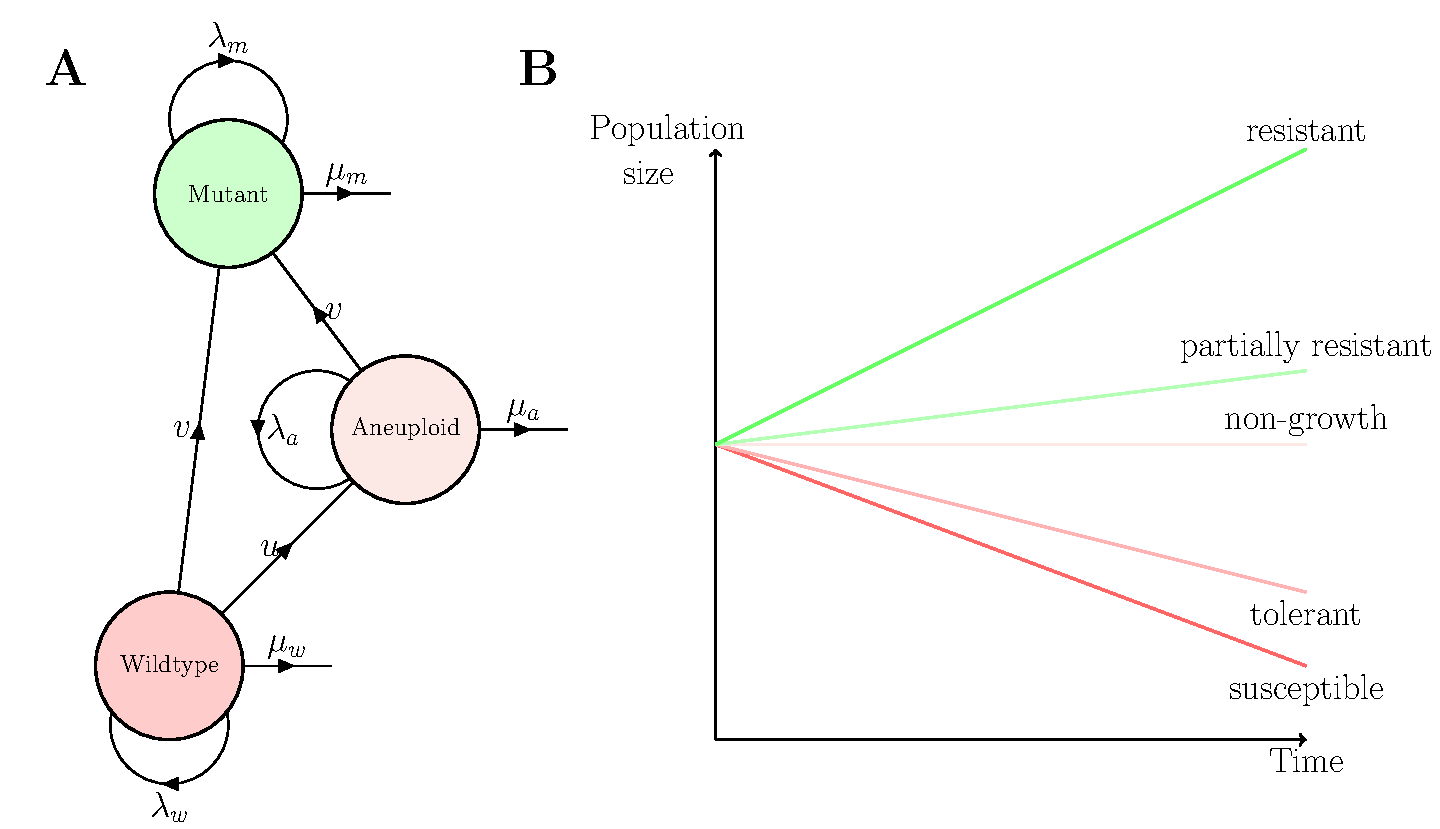
\includegraphics[width=0.5\textwidth]{Figures/figureAneuploidy.pdf}
\caption{
\textbf{Model illustration.}
% TODO in the figure change labels to Wildtype, Aneuploid, Mutant (instead of Euploid etc)
A population of cancer cells is composed of wildtype, aneuploid, and mutant cells, which divide with rates $\lambda_w$, $\lambda_a$, and $\lambda_m$ and die at rates $\mu_w$, $\mu_a$, and $\mu_m$, respectively. 
Wildtype cells can become aneuploid at rate $u$. Both aneuploid and wildtype cells can acquire a beneficial mutation with rate $v$. Color denotes the relative growth rates of the three genotypes such that $\lambda_w - \mu_w < \lambda_a - \mu_a < \lambda_m - \mu_m$.
}
\label{figureAneuploidy}
\end{figure}
%%%%%%%%%%%


%%%%%%%%%%%%%%%%%%%%%%%%%%%%%%%%%%%%%%%%
\subsection*{Evolutionary simulation} 
Simulations are performed using a \emph{Gillespie algorithm} \citep{gillespie1976general,gillespie1977exact} implemented in Python \citep{python}.
The simulation monitors the number of cells of each type: wildtype, aneuploid, and mutant. 
The wildtype population initially consists of $w_0$ cells, whereas the other cell types are initially absent.

\begin{table}
\begin{center}
  \begin{tabular}{| l |p{5cm}| c | c | p{3cm} |}
    \hline
     & Name & Value & Units & References \\ \hline
    $N$ & Initial tumor size & $10^7-10^9$ & cells  & \citet{del2009does} \\ \hline
    $\lambda_w$ & Wildtype division rate& 0.14 & 1/days  & \citep{bozic2013evolutionary} \\ \hline
    $\mu_w$ & Wildtype death rate& 0.17 & 1/days  & \citet{bozic2013evolutionary} \\ \hline
    $\lambda_a$  & Aneuploid division rate$^\ast$ & 0.14 & 1/days  & - \\ \hline
    $\mu_a$ & Aneuploid death rate$^\ast$ & $0.13-0.17$ & 1/days  & - \\ \hline
    $\lambda_m$ & Mutant division rate& 0.14 & 1/days  & \citet{bozic2013evolutionary} \\ \hline
    $\mu_m$ & Mutant death rate& 0.13 & 1/days  & \citet{bozic2013evolutionary} \\ \hline
    $u$ & Missegregation rate& $10^{-3}-10^{-2}$ & 1$\slash$cell division  & \citet{nowak2004evolutionary,bakker2023predicting} \\ \hline
    $v$ & Mutation rate& $10^{-7}-10^{-9}$ &  1$\slash$gene$\slash$cell division  & \citet{nowak2004evolutionary} \\ \hline
  \end{tabular}
\caption{\textbf{Model parameters.} 
Aneuploid birth rate $\lambda_a$ is set to the same value as the wildtype and mutant birth rates, $\lambda_w$ and $\lambda_m$.
Aneuploid death rate $\mu_a$ is set to an intermediate value between the wildtype and mutant death rates, $\mu_w$ and $\mu_m$.}
  \label{table1}
\end{center}
\end{table}

The state of the stochastic system at time $t$ is represented by the triplet $\left(w_t,a_t,m_t\right)$. The following describes the events that may occur (right column), the rates at which they occur (middle column), and the effect these events have on the state (\Cref{figureAneuploidy}):
\begin{subequations}
\begin{flalign*}
(+1,0,0)&:\quad \lambda_ww_t\quad\left(\text{birth of wildtype cell}\right),\\
(-1,0,0)&:\quad \mu_ww_t\quad\left(\text{death of wildtype cell}\right),\\
(-1,+1,0)&:\quad uw_t\quad\left(\text{wildtype cell becomes aneuploid}\right),\\
(-1,0,+1)&:\quad vw_t\quad\left(\text{wildtype cell becomes mutant}\right),\\
(0,+1,0)&:\quad \lambda_aa_t\quad\left(\text{birth of aneuploid cell}\right),\\
(0,-1,0)&:\quad \mu_aa_t\quad\left(\text{death of aneuploid cell}\right),\\
(0,-1,+1)&:\quad va_t\quad\left(\text{aneuploid cell becomes mutant}\right),\\
(0,0,+1)&:\quad \lambda_am_t\quad\left(\text{birth of mutant cell}\right),\\
(0,0,-1)&:\quad \mu_am_t\quad\left(\text{death of mutant cell}\right).
\end{flalign*}
\end{subequations}
Each iteration of the simulation loop starts with computing the rates $\nu_j$ of each event $j$.
We then draw the time until the next event, $\Delta t$, from an exponential distribution whose rate parameter is the sum of the rates of all events, such that $\Delta t \sim \textit{Exp}(\sum_j \nu_j)$.
Then, we randomly determine which event occurred, where the probability for event $j$ is $p_j=\nu_j/\sum_i \nu_i$.
Finally, we update the number of cells of each type according to the event that occurred and update the time from $t$ to $t+\Delta t$. % TODO more details - you need to specify the events and how they change the number of cells. OK
We repeat these iterations until either the population becomes extinct (the number of cells of all types is zero) or the number of mutant cells is high enough so that its extinction probability is $<0.1\%$, that is until
\begin{equation*}
m_t>\left\lfloor-\frac{3\log10}{\log\left(\frac{\mu_m}{\lambda_m}\right)}\right\rfloor+1,
\end{equation*}

\paragraph{$\tau$-leaping.}
% TODO "is large" - how large?
When the size of the initial population is large we utilize $\tau$-leaping \citep{gillespie2001approximate}, where change in number of cells of genotype $i$ in a fixed time interval $\Delta t$ is Poisson distributed with mean $\nu_i\Delta t$.
If the increment is negative and larger then the subpopulation size then updated to be zero. % TODO "and larger..."??

\paragraph{Density-dependent growth.}

In our analysis we assume that lineages produced by cells from the initial population divide and die independently of each other, which may be unrealistic, as cells usually compete for resources.
A more realistic model includes competition for limited resources and spatial structure, which may play an important role in the development of cancer \citep[e.g.,][]{martens2011spatial}.
To simulate birth and death rates that depend on the number of cells in the population, we transform the rates of division and death to the following:
\begin{align*}
\lambda_w' &= \lambda_w, \\
\mu_w' &= \mu_w,\\
\lambda_a' &= C_1+\left(\lambda_a-\mu_a\right)\left(1-\frac{w+a+m}{K}\right),\\ 
\mu_a' &= C_1,\\
\lambda_m' &= C_2+\left(\lambda_m-\mu_m\right)\left(1-\frac{w+a+m}{K}\right),\\ 
\mu_m' &= C_2,
\end{align*}
where $C_1, C_2>0$ are constants. % TODO what constants?

%%%%%%%%%%%%%%%%%%%%%%%%%%%%%%%%%%%%%%%%
\subsection*{Code and data availability.} All source code is available online at \url{https://github.com/yoavram-lab/EvolutionaryRescue}.

%\newpage
\section*{Results}

% TODO: OVERVIEW OF RESULTS 

%%%%%%%%%%%%%%%%%%%%%%%%%%%%%%%%%%%%%
\subsection*{Survival probability}

To analyze evolutionary rescue in this model, we use the framework of \emph{multitype branching processes} \citep{rybnikov2021fitness,harris1963theory}. 
This allows us to find explicit expressions for the \emph{survival probability}: the probability that a lineage descended from a single cell does not become extinct.

Let $p_w$, $p_a$, and $p_m$ be the survival probabilities of a population consisting initially of single wildtype cell, aneuploid cell, or mutant cell, respectively.
The complements $1-p_w$, $1-p_a$, and $1-p_m$ are the extinction probabilities, which satisfy each its respective equation,
\begin{equation} \label{extinction_prob}
\begin{aligned}
1-p_w = &\frac{\mu_w}{\lambda_w+\mu_w+u+v} + 
		  \frac{u}{\lambda_w+\mu_w+u+v}\left(1-p_a\right) + \\
		  & \frac{\lambda_w}{\lambda_w+\mu_w+u+v}\left(1-p_w\right)^2 +
		  \frac{v}{\lambda_w+\mu_w+u+v}\left(1-p_m\right) ,\\
1-p_a = &\frac{\mu_a}{\lambda_a+\mu_a+v}+\frac{v}{\lambda_a+\mu_a+v}\left(1-p_m\right)+\frac{\lambda_a}{\lambda_a+\mu_a+v}\left(1-p_a\right)^2 ,\\
1-p_m = &\frac{\mu_m}{\lambda_m+\mu_m}+\frac{\lambda_m}{\lambda_m+\mu_m}\left(1-p_m\right)^2 .	 
\end{aligned}
\end{equation}

The survival probabilities are given by the smallest solution for each quadratic equation \citep{uecker2015adaptive}. Therefore we have
\begin{equation}\label{survival_prob}
\begin{aligned}
p_w &= \frac{\lambda_w-\mu_w-u-v+\sqrt{\left(\lambda_w-\mu_w-u-v\right)^2+4\lambda_w\left(up_a+vp_m\right)}}{2\lambda_w} ,\\
p_a &= \frac{\lambda_a-\mu_a-v+\sqrt{\left(\lambda_a-\mu_a-v\right)^2+4\lambda_avp_m}}{2\lambda_a}, \\
p_m &= \frac{\lambda_m-\mu_m}{\lambda_m} .
\end{aligned} 
\end{equation}
Note that the equation for $p_w$ depends on both $p_a$ and $p_m$, and the equation for $p_a$ depends on $p_m$.
To proceed, we can plug the solution for $p_m$ and $p_a$ into the solution for $p_w$. We perform this for three different scenarios.

%%%%%%%%%%%%%%%%%%%%%%%%%%%%%%%%%%%%%
\subsubsection*{Scenario 1: Aneuploid cells are partially resistant} 

We first assume that aneuploidy provides partial resistance to drug therapy, $\lambda_a>\mu_a$, and that this resistance is significant, $\left(\lambda_a-\mu_a-v\right)^2 > 4\lambda_a v p_m$.
We thus rewrite \cref{survival_prob} as
\begin{align*}
p_w&=\frac{\lambda_w-\mu_w-u-v}{2\lambda_w}\left(1-\sqrt{1+\frac{4\lambda_w\left(vp_m+up_a\right)}{\left(\lambda_w-\mu_w-u-v\right)^2}}\right) ,
\text{and} \\
p_a&=\frac{\lambda_a-\mu_a-v}{2\lambda_a}\left(1+\sqrt{1+\frac{4\lambda_avp_m}{\left(\lambda_a-\mu_a-v\right)^2}}\right) . 
\end{align*}
Using the quadratic Taylor expansion $\sqrt{1+x}=1+x/2+O(x^2)$ and assuming $u,v \ll 1$,
we obtain the following approximation for the survival probability of a population initially consisting of a single wildtype cell,
\begin{align}\label{survprobwapprox1}
p_w 
&\approx -\frac{vp_m+up_a}{\lambda_w-\mu_w-u-v}\\
\nonumber
%&\approx-\frac{1}{\lambda_w-\mu_w-u-v}\left[\frac{v\left(\lambda_a-\mu_a-u\right)}{\lambda_a}+\frac{uv\left(\lambda_m-\mu_m\right)}{\lambda_m\left(\lambda_a-\mu_a-u\right)}+\frac{v\left(\lambda_m-\mu_m\right)}{\lambda_m}\right]\\ \label{survprobw2}
&\approx-\frac{1}{\lambda_w-\mu_w}\left[\frac{u\left(\lambda_a-\mu_a\right)}{\lambda_a}+\frac{uv\left(\lambda_m-\mu_m\right)}{\lambda_m\left(\lambda_a-\mu_a\right)}+\frac{v\left(\lambda_m-\mu_m\right)}{\lambda_m}\right]\\
\end{align}

%%%%%%%%%%%%%%%%%%%%%%%%%%%%%%%%%%%%%
\paragraph{Second-order approximation.} % TODO consider moving to Appendix
To improve our approximation, we can consider the second term of the Taylor series expansion,
\begin{align*}
\left(1+\frac{4\lambda_avp_m}{\left(\lambda_a-\mu_a-v\right)^2}\right)^{\frac{1}{2}}=1+\frac{2\lambda_avp_m}{\left(\lambda_a-\mu_a-v\right)^2}-\frac{\left(\lambda_avp_m\right)^2}{4\left(\lambda_a-\mu_a-v\right)^4}+\cdots,
\end{align*}
which gives us the following approximation,
\begin{align}
p_a \approx \frac{\lambda_a-\mu_a-v}{\lambda_a}+\frac{vp_m}{\lambda_a-\mu_a-v}-\frac{\lambda_a\left(vp_m\right)^2}{8\left(\lambda_a-\mu_a-v\right)^3} .
\end{align}
We therefore have
\begin{align}\nonumber
p_w&\approx-\frac{1}{\lambda_w-\mu_w-u-v}\left[\frac{u\left(\lambda_a-\mu_a-v\right)}{\lambda_a}+\frac{uv\left(\lambda_m-\mu_m\right)}{\lambda_m\left(\lambda_a-\mu_a-v\right)}+\frac{v\left(\lambda_m-\mu_m\right)}{\lambda_m}-\frac{uv^2\lambda_a\left(\lambda_m-\mu_m\right)^2}{8\lambda_m^2\left(\lambda_a-\mu_a-v\right)^3}\right]\\ \label{survprobw3}
&\approx-\frac{1}{\lambda_w-\mu_w}\left[\frac{u\left(\lambda_a-\mu_a\right)}{\lambda_a}+\frac{uv\left(\lambda_m-\mu_m\right)}{\lambda_m\left(\lambda_a-\mu_a\right)}+\frac{v\left(\lambda_m-\mu_m\right)}{\lambda_m}-\frac{uv^2\lambda_a\left(\lambda_m-\mu_m\right)^2}{8\lambda_m^2\left(\lambda_a-\mu_a\right)^3}\right], 
\end{align}
and using $\Delta_k=\lambda_k-\mu_k$, we can write the above equation as
\begin{equation}\label{survprobwapproxcorrected}
p_w \approx -\frac{1}{\Delta_w}\left(\frac{u\Delta_a}{\lambda_a}+\frac{uv\Delta_m}{\lambda_m\Delta_a}+\frac{v\Delta_m}{\lambda_m}-\frac{uv^2\lambda_a\Delta_m^2}{8\lambda_m^2\Delta_a^3}\right).
\end{equation}


%%%%%%%%%%%%%%%%%%%%%%%%%%%%%%%%%%%%%
\subsubsection*{Scenario 2: Aneuploid cells are tolerant.} 

We now assume that aneuploidy provides tolerance to drug therapy, that is, the number of aneuploid cells significantly declines over time, but at a lower rate than the number of wildtype cells, $\lambda_w - \mu_w < \lambda_a - \mu_a < 0$. We also assume that the decline are significant, $\left(\lambda_a-\mu_a-v\right)^2 > 4\lambda_a v p_m$.
We rewrite \cref{survival_prob} as
\begin{align*}
p_w&=\frac{\lambda_w-\mu_w-u-v}{2\lambda_w}\left(1-\sqrt{1+\frac{4\lambda_w\left(vp_m+up_a\right)}{\left(\lambda_w-\mu_w-u-v\right)^2}}\right) ,
\text{and} \\
p_a&=\frac{\lambda_a-\mu_a-v}{2\lambda_a}\left(1-\sqrt{1+\frac{4\lambda_avp_m}{\left(\lambda_a-\mu_a-v\right)^2}}\right) .
\end{align*}
Since $u,v\ll1$, this can be approximated by % TODO how do you do the first approx? taylor?
\begin{equation}\label{survprobwinitial}
\begin{aligned}
p_w&\approx-\frac{vp_m+up_a}{\lambda_w-\mu_w-u-v}\\
&\approx\frac{1}{\lambda_w-\mu_w-u-v}\left[\frac{uv\left(\lambda_m-\mu_m\right)}{\lambda_m\left(\lambda_a-\mu_a-v\right)}-\frac{v\left(\lambda_m-\mu_m\right)}{\lambda_m}\right]\\ %\label{survprobw2}
&\approx\frac{v\left(\lambda_m-\mu_m\right)}{\lambda_m\left(\lambda_w-\mu_w\right)}\left[\frac{u}{\left(\lambda_a-\mu_a\right)}-1\right]\\
%&=\frac{v\Delta_m}{\lambda_m\Delta_w}\left(\frac{u}{\Delta_a}-1\right) .
\end{aligned}
\end{equation}
%Using the notational convention
%\begin{equation}\label{notationalconv}
%\Delta_i=\lambda_i-\mu_i,
%\end{equation}
%we write \eqref{survprobw} as
%\begin{equation}\label{survprobwapprox2}
%p_w=\frac{v\Delta_m}{\lambda_m\Delta_w}\left(\frac{u}{\Delta_a}-1\right).
%\end{equation}

%%%%%%%%%%%%%%%%%%%%%%%%%%%%%%%%%%%%%
\subsubsection*{Scenario 3: Aneuploid cells are non-growing} % TODO consider this name

We now assume that the growth rate of aneuploid cells is close to zero (either positive or negative), such that  $\left(\lambda_a-\mu_a-v\right)^2 < 4\lambda_avp_m$.
We rewrite \cref{survival_prob} as
\begin{equation}
p_a=\frac{\lambda_a-\mu_a-v+2\sqrt{\lambda_a vp_m}\left(1+\frac{\left(\lambda_a-\mu_a-v\right)^2}{4\lambda_avp_m}\right)^{\frac12}}{2\lambda_a} .
\end{equation}
Using a following Taylor series expansion
\begin{equation*}
\left(1+\frac{\left(\lambda_a-\mu_a-v\right)^2}{4\lambda_avp_m}\right)^{\frac{1}{2}}=1+\frac{\left(\lambda_a-\mu_a-v\right)^2}{8\lambda_avp_m}+\cdots,
\end{equation*}
we obtain the approximation
\begin{equation}
\begin{aligned}
p_a&\approx\frac{\lambda_a-\mu_a-v+2\sqrt{\lambda_a vp_m}\left[1+\frac{\left(\lambda_a-\mu_a-v\right)^2}{8\lambda_avp_m}\right]}{2\lambda_a}\\
&=\frac{\lambda_a-\mu_a-v+2\sqrt{\lambda_a vp_m}+\frac{\left(\lambda_a-\mu_a-v\right)^2}{4\sqrt{\lambda_avp_m}}}{2\lambda_a}\\
&=\frac{\left(\lambda_a-\mu_a-v+2\sqrt{\lambda_avp_m}\right)^2+4\lambda_avp_m}{8\lambda_a\sqrt{\lambda_avp_m}}\\
&=\frac{4\lambda_avp_m+4\lambda_avp_m\left(1+\frac{\lambda_a-\mu_a-v}{2\sqrt{\lambda_avp_m}}\right)^2}{8\lambda_a\sqrt{\lambda_avp_m}}\\
&=\frac{1}{2\lambda_a}\left(\lambda_a-\mu_a-v+2\sqrt{\lambda_avp_m}\right).
\end{aligned}
\end{equation}
From \Cref{survprobwinitial}, % TODO I dont see how the referred equation plays a part here
the survival probability of a population starting from one wildtype individual is
\begin{equation}\label{scenario3}
\begin{aligned}
p_w&\approx-\frac{1}{\lambda_w-\mu_w-u-v}\left[v\frac{\lambda_m-\mu_m}{\lambda_m}+\frac{u}{2\lambda_a}\left(\lambda_a-\mu_a-v+2\sqrt{\lambda_avp_m}\right)\right]\\
&=-\frac{1}{\lambda_w-\mu_w-u-v}\left[v\frac{\lambda_m-\mu_m}{\lambda_m}+\frac{u}{2\lambda_a}\left(\lambda_a-\mu_a-v\right)+u\sqrt{\frac{v\left(\lambda_m-\mu_m\right)}{\lambda_a\lambda_m}}\right].
%&=-\frac{1}{\Delta_w-u-v}\left[v\frac{\Delta_m}{\lambda_m}+\frac{u\left(\Delta_a-v\right)}{2\lambda_a}+u\sqrt{\frac{v\Delta_m}{\lambda_a\lambda_m}}\right],
\end{aligned}
\end{equation}


%%%%%%%%%%%%%%%%%%%%%%%%%%%%%%%%%%%%%
\subsection*{Evolutionary rescue probability}

Evolutionary rescue occurs when mutant cells appear and fixate ($m_t>>1$) in the population before the population becomes extinct ($w_t=a_t=m_t=0$).
Aneuploidy may contribute to evolutionary rescue by either preventing (when $\Delta_a>0$) or delaying (when $0>\Delta_a>\Delta_w$) the extinction of the population before mutant cells appear and fixate.

To estimate the rescue probability $p_{rescue}$, we assume independence between clonal lineages starting from an initial population of $N$ wildtype cells.
Thus, the rescue probability is given by 
\begin{equation}
p_{rescue}=1-\left(1-p_w\right)^N\approx 1-\e^{-Np_w} ,
\end{equation}
where the approximation $(1-p_w)\approx e^{-p_w}$ assumes that $p_w$ (but not $N p_w$) is small.

Now, we apply the approximations for the survival probability $p_w$ from \Cref{survprobwapprox1,survprobwinitial,scenario3}. Therefore, substituting $\Delta_k=\lambda_k-\mu_k$ , the rescue probability is given by
\begin{equation}\label{rescue_prob}
p_{rescue} = \left\{
  \begin{array}{@{}ll@{}}
  1-\exp\left[\frac{N}{\Delta_w-u-v}\left(v\frac{\Delta_m}{\lambda_m}+\frac{u\left(\Delta_a-v\right)}{2\lambda_a}+u\sqrt{\frac{v\Delta_m}{\lambda_a\lambda_m}}\right)\right],\quad\text{if }4\lambda_avp_m>\left(\Delta_a-v\right)^2,\\
   1-\exp\left[\frac{v\Delta_mN}{\lambda_m\Delta_w}\left(1-\frac{u}{\Delta_a}\right)\right],\quad\text{if }\Delta_a<0\quad\text{and}\quad4\lambda_avp_m<\left(\Delta_a-v\right)^2,\\
   1-\exp\left[\frac{N}{\Delta_w}\left(\frac{u\Delta_a}{\lambda_a}+\frac{uv\Delta_m}{\lambda_m\Delta_a}+\frac{v\Delta_m}{\lambda_m}\right)\right],\quad\text{if }\Delta_a>0\quad\text{and}\quad4\lambda_avp_m<\left(\Delta_a-v\right)^2.
  \end{array}\right.
\end{equation}

%Note that if instead \cref{survprobwapprox1} we apply \cref{survprobwapproxcorrected}, we have
%\begin{align}\label{survprobresistantaneuploidy}
%p_{rescue}=1-\left(1-p_w\right)^N\approx 1-\e^{-Np_w}=1-\exp\left[\frac{N}{\Delta_w}\left(\frac{u\Delta_a}{\lambda_a}+\frac{uv\Delta_m}{\lambda_m\Delta_a}+\frac{v\Delta_m}{\lambda_m}-\frac{uv^2\lambda_a\Delta_m^2}{8\lambda_m^2\Delta_a^3}\right)\right].
%\end{align}

In \Cref{SurvPlot,SurvPlotLargeN} we explore the effects of the wildtype and aneuploid growth rates on the rescue probability for small and large population sizes ($N=10^4$ and $N=10^8$, respectively).

\Cref{SurvPlotNData} show $p_{rescue}$ as a function of $N$, including comparison of our first approximation \eqref{aneuploidyresistentfirstapprox} and simulation results.

\Cref{P_est,P_est_large_N} show the rescue probability for initial population sizes $N=10^4$ and $N=10^8$, respectively. % TODO check figure refs

In \Cref{DeleteriousPlot}, we compare the exact result (\cref{survival_prob}) with numerical simulations. The transition between the regimes defined by \cref{AneuploidyDeleteriousApprox} and \cref{pestthirdcase} respectively occurs at:
\begin{align}\label{thresholdvalueaneuploid}
\Delta_a^*=2vp_m+v+2\sqrt{vp_m\left(vp_m+\mu_a+v\right)}.
\end{align}


%%%%%%%%%%%%%%%%%%%%%%%%%%%%%%%%%%%%%%%%%%%%%%%%%%%%%%%%%%%%
\paragraph*{Density-dependent growth}

We perform stochastic simulations for different values of the carrying capacity $K$ and we plot the results in Figure \ref{SurvPlotNDataLogisticKComplete}.  We observe that as $K$ increases the simulations converge to the analytic result which is because the carrying capacity is much larger then the population size of aneuploid cells for which the probability that the population is rescued is certain.


%%%%%%%%%%%%%%%%%%%%%%%%%%%%%%%%%%%%%%%%%%%%%%%%%%%%%%%%%%%%
\subsection*{Standing genetic variation}

So far we have assumed that the initial population of cells consisted entirely of wildtype cells.
We now modify this assumption so that the initial population includes a fraction $f$ of cells with aneuploidy.
The probability of evolutionary rescue by cells with aneuploidy from the initial population is
\begin{equation*}
p_{old} = 1-\left(1-p_a\right)^{fN}\approx 1-\e^{-fNp_a}.
\end{equation*}
The total probability of evolutionary rescue is given by
\begin{align}\nonumber
p_{total} 	&= p_{new}+\left(1-p_{new}\right)p_{old}\\
			&= 1-\exp\left(-\left[\left(1-f\right)p_w + fp_a\right]N\right) .
\end{align}

The fraction of cases in which the population is rescued by the standing genetic variation is given by $F\left(f\right)=\frac{p_{old}}{p_{total}}$.
%=\frac{ 1-\e^{-fNp_a}}{1-\e^{-\left[\left(1-f\right)p_w+fp_a\right]N}}.
Setting $F=\frac{1}{2}$, we use the expansion $\e^x \approx 1+x$ to obtain
\begin{equation}\label{halfeqstandvar}
f^*\approx\frac{p_w}{p_w+p_a}.
\end{equation}
See \Cref{FractionPlot} for a demonstration of $F$ and $f*$.

%%%%%%%%%%%%%%%%%%%%%%%%%%%%%%%%%%%%%%%%%%
\subsection*{Contribution of aneuploidy to the evolutionary rescue of cancer}
We wish to understand the contribution of aneuploidy to evolutionary rescue of the cancer cell population. For this purpose we define the ratio of the probability of evolutionary rescue when aneuploidy can play a role in rescue ($u>0$) to the probability where acquisition of aneuploidy is not possible ($u=0$):
\begin{equation}\label{ratiorescueexact}
H=\frac{\left.p_{rescue}\right|_{u>0}}{\left.p_{rescue}\right|_{u=0}}.
\end{equation}
As a result, we obtain from \eqref{rescue_prob} the approximation for the ratio:
\begin{equation}\label{ratiorescue}
H\sim\left\{
  \begin{array}{@{}ll@{}}
  \frac{1-\exp\left[\frac{N}{\Delta_w-u-v}\left(v\frac{\Delta_m}{\lambda_m}+\frac{u\left(\Delta_a-v\right)}{2\lambda_a}+u\sqrt{\frac{v\Delta_m}{\lambda_a\lambda_m}}\right)\right]}{1-\exp\left[\frac{vN\Delta_m}{\left(\Delta_w-v\right)\lambda_m}\right]},\quad\text{if }4\lambda_avp_m>\left(\Delta_a-v\right)^2,\\
   \frac{1-\exp\left[\frac{v\Delta_mN}{\lambda_m\Delta_w}\left(1-\frac{u}{\Delta_a}\right)\right]}{1-\exp\left(\frac{v\Delta_mN}{\lambda_m\Delta_w}\right)},\quad\text{if }\Delta_a<0\quad\text{and}\quad4\lambda_avp_m<\left(\Delta_a-v\right)^2,\\
   \frac{1-\exp\left[\frac{N}{\Delta_w}\left(\frac{u\Delta_a}{\lambda_a}+\frac{uv\Delta_m}{\lambda_m\Delta_a}+\frac{v\Delta_m}{\lambda_m}\right)\right]}{1-\exp\left[\frac{v\Delta_mN}{\lambda_m\Delta_w}\right]},\quad\text{if }\Delta_a>0\quad\text{and}\quad4\lambda_avp_m<\left(\Delta_a-v\right)^2. % TODO this term can be simplified/approximated
  \end{array}\right.
\end{equation}

%\begin{equation}
%H\sim\left\{
%  \begin{array}{@{}ll@{}}
%  \frac{1-\exp\left[\frac{N}{\Delta_w-u-v}\left(v\frac{\Delta_m}{\lambda_m}+\frac{u\left(\Delta_a-v\right)}{2\lambda_a}+u\sqrt{\frac{v\Delta_m}{\lambda_a\lambda_m}}\right)\right]}{1-\exp\left[\frac{vN\Delta_m}{\left(\Delta_w-v\right)\lambda_m}\right]},\quad\text{if }4\lambda_avp_m>\left(\Delta_a-v\right)^2,\\
%   \frac{1-\exp\left[\frac{v\Delta_mN}{\lambda_m\Delta_w}\left(1-\frac{u}{\Delta_a}\right)\right]}{1-\exp\left(\frac{v\Delta_mN}{\lambda_m\Delta_w}\right)},\quad\text{if }\Delta_a<0\quad\text{and}\quad4\lambda_avp_m<\left(\Delta_a-v\right)^2,\\
%   \frac{1-\exp\left(\frac{u\Delta_aN}{\lambda_a\Delta_w}\right)}{1-\exp\left(\frac{v\Delta_mN}{\lambda_m\Delta_w}\right)},\quad\text{if }\Delta_a>0\quad\text{and}\quad4\lambda_avp_m<\left(\Delta_a-v\right)^2.
%  \end{array}\right.
%\end{equation}
We plot \eqref{ratiorescue} in Figure \ref{RatioEvolRescue} for both resistent and susceptible aneuploidy as a function of the proliferation rate of the wildtype cells and in Figure \ref{RatioEvolRescuePopulationSize} as a function of the initial population size of wildtype cells.


%%%%%%%%%%%%%%%%%%%%%%%%%%%%%%%%%%%%
\subsection*{Rescue time}
We calculate the mean time for the appearance of the first mutant that rescues the cancer cell population. This can occur either through the pathway $wildtype\rightarrow aneuploid \rightarrow mutant$ or through the pathway $wildtype \rightarrow mutant$. We start with the second pathway: let $T_1$ be the time at which the first mutant cell appears which rescues the population when evolutionary rescue is only possible through mutation. We are interested in the mean time $\tau_1=\mathbb{E}\left[T_1\right]$.

% something is missing in the next line...?
% the entire section is missing text...

The number of successful mutants generated until time $t$ can be approximated by a inhomogeneous Poisson process with rate $R\left(t\right)=up_aw_t$
%\begin{align}
%\tau_1\sim \text{Poisson}\left(\frac{1}{up_aw_t}\right),
%\end{align}
where $w_t$ is the size of the wildtype population at time $t$: 
\begin{equation}
w_t=N\e^{\Delta_wt}.
\end{equation}
We are interested in the time to appearance of the first successful mutant cell conditional on population surviving:
\begin{align*}
P\left(T_1<t\right)&=P\left(T_1<t|m_{t\rightarrow\infty}\neq0\right)P\left(m_{t\rightarrow\infty}\neq0\right)\\
&+P\left(T_1<t|m_{t\rightarrow\infty}=0\right)P\left(m_{t\rightarrow\infty}=0\right).
\end{align*}
As a result, the cumulative distribution function can be written as:
\begin{align*}
P\left(T_1<t\right)&=P\left(T_1<t|m_{t\rightarrow\infty}\neq0\right)P\left(m_{t\rightarrow\infty}\neq0\right),
\end{align*}
where we used the fact that evolutionary rescue is impossible when the mutant population is destined to be zero:
\begin{align*}
P\left(T_1<t|m_{t\rightarrow\infty}=0\right)=0.
\end{align*}
As a result, we obtain 
\begin{align}
P\left(T_1<t|m_{t\rightarrow\infty}\neq0\right)=\frac{P\left(\tau_1<t\right)}{1-\left(1-p_w\right)^N},
\end{align}
where we have used
\begin{equation}
P\left(m_{t\rightarrow\infty}\neq0\right)=1-\left(1-p_w\right)^N.
\end{equation}
The probability density function of $T_1$ is given by:
\begin{align}
f_{T_1}\left(t_1\right)=R\left(t_1\right)\e^{-\int_0^{t_1} R(t)\d t}.
\end{align}
As a result, the time $T_1$ conditional on evolutionary rescue is given by:
\begin{align}
f_{T_1}\left(t_1|m_{t\rightarrow\infty}\neq0\right)=\frac{R\left(t_1\right)\e^{-\int_0^{t_1} R(t)\d t}}{1-\left(1-p_w\right)^N}.
\end{align}
The expectation of $T_1$ is:
\begin{align}\label{meantime1}
\tau_1=\mathbb{E}\left[T_1\right]&=\frac{\int_0^\infty\e^{-\int_0^\tau R(t)\d t}\d\tau}{1-\left(1-p_w\right)^N}=\frac{\int_0^\infty\e^{-uNp_a\frac{\e^{\Delta_w\tau}-1}{\Delta_w}}\,\d\tau}{1-\left(1-p_w\right)^N}.
\end{align}
The fration in exponential of the integrand in \eqref{meantime1} can approximated as:
\begin{equation*}
\frac{\e^{\Delta_w\tau}-1}{\Delta_w}=\frac{1+\Delta_w\tau+O(\tau^2)-1}{\Delta_w}=\tau+O(\tau^2).
\end{equation*}
As a result, the mean time $\tau_1$ can be simplified:
\begin{align}\label{limitapprox}
\tau_1\approx\left(1+\e^{-Np_w}\right)\int_0^\infty\e^{-uNp_a\tau}\,\d\tau=\frac{\left(1+\e^{-Np_w}\right)}{uNp_a},
\end{align}
where in the previous line we have used the approximation:
\begin{equation*}
\frac{1}{1-\e^{-Np_w}}\approx1+\e^{-Np_w}.
\end{equation*}
We plot the expansion \eqref{limitapprox} in Figure \ref{MeanTimeGrowthAneuploidyPlot} and observe that it is a very good fit for intermediate and large values of the initial wildtype population size.

%Let $T=T_1+T_2$ be the time the first mutant cell that appears and rescues the population, where $T_1$ is the time at which the first aneuploid cell appears whose lineage will rescue the population and $T_2$ the time for this aneuploidy lineage to produce the first mutant that rescues the population. The expected mean time $\tau_1=\mathbb{E}\left[T_1\right]$ is identical to \eqref{meantime1} with adequate parameters.
%
%For an aneuploid cell, let $a_\tau$ be the number of its aneuploid descendents at time $\tau$. Each of these descentends have a probability $v\d \tau$ of producing a mutant which has a probability $p_m$ to survive. Consequently, the probability that the lineage descendent from a single aneuploid cell produces succesful mutant in the time interval $\left[\tau,\tau+\d \tau\right]$ is $vp_ma_t\d \tau$. Since the number of succesful mutants is a Poisson process, the probability of evolutionary rescue occurring until time $t$, given $a_\tau$, is given by:
%\begin{align}
%1-\exp\left(-\int_0^t vp_ma_\tau\d \tau\right)=1-\exp\left(-vp_mA_t\right),
%\end{align}
%where $A_t$ is the weight of the lineage until time $t$, defined as:
%\begin{equation}
%A_t=\int_0^t a_\tau\d \tau.
%\end{equation}
%As a result, to obtain $p_a\left(t\right)$ we average over all possible values of $A_t$:
%\begin{align}
%p_a\left(t\right)&=\int_0^\infty \d a P\left(A_T=a\right)\left[1-\e^{-vp_mA_t}\right]\\
%&=1-\mathbb{E}\left[\e^{-vp_mA_t}\right]
%\end{align}
%Following the steps outlines in \citep{weissman2009rate} we obtain:
%\begin{align}
%p_a\left(t\right)=\frac{\left(a_+-1\right)\left(1-a_-\right)\left(1-\e^{-\left(1-\delta\right)\left(a_+-a_-\right)t}\right)}{a_+-1+\left(1-a_-\right)\e^{-\left(1-\delta\right)\left(a_+-a_-\right)t}},
%\end{align}
%where
%\begin{align}
%a_\pm=\frac{2-\delta-vp_m\pm\sqrt{\left(\delta+vp_m\right)^2-4vp_m}}{2\left(1-\delta\right)}.
%\end{align}
%and
%\begin{align}
%\delta=\frac{\Delta_a}{\Delta_w}
%\end{align}
%
%The cumulative distribution of $T_2$ is given by $\frac{p_a\left(t\right)}{p_m}$ from which we obtain the mean time:
%\begin{align}
%\tau_2=\mathbb{E}\left[T_2\right]=\int_0^\infty\left(1-\frac{p_a\left(t\right)}{p_a}\right)\d t.
%\end{align}

%%%%%%%%%%%%%%%%%%%%%%%%%%%%%%%%%%%%%%%%%%
When $Nu\gg1$ the aneuploid population can be assumed to be deterministic and approximated by the solution to the system of ODEs:
\begin{equation}
a_t=\frac{Nu\e^{\Delta_wt}}{\Delta_w-\Delta_a}\left[1-\e^{\left(\Delta_w-\Delta_a\right)t}\right].
\end{equation}
As a result, when $N\gg1$ the number of successful mutants created by direct mutation or though aneuploidy are an inhomogeneous Poisson processes with the rates:

%\begin{align}
%f_{T_2}\left(t_2|m_{t\rightarrow\infty}\neq0\right)=\frac{R_2\left(t_2\right)\e^{-\int_0^{t_2} R_2(t)\d t}}{1-\left(1-p_w\right)^N}
%\end{align}

%\begin{align}\label{meantime2}
%\tau_2=\mathbb{E}\left[T_2\right]&=\frac{\int_0^\infty\e^{-\int_0^\tau R_2(t)\d t}\d\tau}{1-\left(1-p_w\right)^N}=\frac{\int_0^\infty\e^{-uNp_a\frac{\e^{\Delta_w\tau}-1}{\Delta_w}}\,\d\tau}{1-\left(1-p_w\right)^N}.
%\end{align}
%
%\begin{align}\label{meantime3}
%\tau_3=\frac{\int_0^\infty\e^{-vNp_m\frac{\e^{\Delta_w\tau}-1}{\Delta_w}}\,\d\tau}{1-\left(1-p_w\right)^N}.
%\end{align}

\begin{align*}
r_1\left(t\right)&=vp_m\int_0^ta_{\tau}\,\d\tau=\frac{uvNp_m}{\Delta_w-\Delta_a}\left(\frac{\e^{\Delta_wt}-1}{\Delta_w}-\frac{\e^{\Delta_at}-1}{\Delta_a}\right),\\
r_2\left(t\right)&=vp_m\int_0^tw_{\tau}\,\d\tau=vNp_m\frac{\e^{\Delta_w\tau}-1}{\Delta_w}.
\end{align*}
For large initial population sizes we can assume that both rescue mutations produced through direct mutation and aneuploidy are independent and, as a result, they can be merged into a single Poisson process with rate $\left(r_1+r_2\right)\left(t\right)$. Consequently, the mean time to the appearance of the first rescue mutant is: 
\begin{align}\label{meantimet2}
\tau_2=\frac{\int_0^\infty\e^{-\left(r_1+r_2\right)}\,\d\tau}{1-\left(1-p_w\right)^N}=\frac{\int_0^\infty\exp\left[-\frac{uvNp_m}{\Delta_w-\Delta_a}\left(\frac{\e^{\Delta_w\tau}-1}{\Delta_w}-\frac{\e^{\Delta_a\tau}-1}{\Delta_a}\right)-vNp_m\frac{\e^{\Delta_w\tau}-1}{\Delta_w}\right]\,\d\tau}{1-\left(1-p_w\right)^N},
\end{align}
which we plot in Figure \ref{MeanTimeDeleteriousAneuploidyPlot} as a function of the initial population size.

We wish to obtain a simpler formula for $\tau_2$ in an analogous way to \eqref{limitapprox}. For this, we make use of the following expansions:
\begin{align*}
\frac{\e^{\Delta_w\tau}-1}{\Delta_w}&=\frac{1+\Delta_w\tau+\frac{\Delta_w^2\tau^2}{2}+O(\tau^3)-1}{\Delta_w}=\tau+\frac{\Delta_w}{2}\tau^2+O(\tau^3).\\
\frac{\e^{\Delta_a\tau}-1}{\Delta_a}&=\frac{1+\Delta_a\tau+\frac{\Delta_a^2\tau^2}{2}+O(\tau^3)-1}{\Delta_a}=\tau+\frac{\Delta_w}{2}\tau^2+O(\tau^3),
\end{align*}
which allow us to write:
\begin{equation*}
\frac{\e^{\Delta_w\tau}-1}{\Delta_w}-\frac{\e^{\Delta_a\tau}-1}{\Delta_a}\approx\frac{\left(\Delta_w-\Delta_a\right)\tau^2}{2}.
\end{equation*}
As a result, the integrand in \eqref{meantimet2} can be written as:
\begin{align*}
&\exp\left[-\frac{uvNp_m}{\Delta_w-\Delta_a}\left(\frac{\e^{\Delta_w\tau}-1}{\Delta_w}-\frac{\e^{\Delta_a\tau}-1}{\Delta_a}\right)-vNp_m\frac{\e^{\Delta_w\tau}-1}{\Delta_w}\right]\approx\exp\left(-uvNp_m\tau^2-vNp_m\tau\right)\\
&=\exp\left(\frac{vNp_m}{2}\right)\exp\left[-\frac{uvNp_m}{2}\left(\tau+\frac{1}{u}\right)\right].
\end{align*}
Consequently, the mean time $\tau_2$ is obtained to be:
\begin{align}\label{limitapprox2}
\tau_2\approx\left[1+\exp\left(-Np_w\right)\right]\exp\left(\frac{vNp_m}{2u}\right)\frac{\erfc\left(\sqrt{\frac{vNp_m}{2u}}\right)}{\sqrt{\frac{2uvNp_m}{\pi}}},
\end{align}
where $\erfc$ is the complementary error function. We plot the expansion \eqref{limitapprox2} in Figure \ref{MeanTimeDeleteriousAneuploidyPlot} and observe that it is a very good fit for large values of the initial wildtype population size.

If we select only linear terms in the following expansions:
\begin{align*}
\frac{\e^{\Delta_w\tau}-1}{\Delta_w}&=\frac{1+\Delta_w\tau+O(\tau^2)-1}{\Delta_w}=\tau+O(\tau^2).\\
\frac{\e^{\Delta_a\tau}-1}{\Delta_a}&=\frac{1+\Delta_a\tau+O(\tau^2)-1}{\Delta_a}=\tau+O(\tau^2),
\end{align*}
we obtain the first order approximation for $\tau_2$:
\begin{align}\label{limitapprox3}
\tau_2\approx\left(1+\e^{-Np_w}\right)\int_0^\infty\e^{-uNp_m\tau}\,\d\tau=\frac{\left(1+\e^{-Np_w}\right)}{uNp_m},
\end{align}
which we plot in Figure \ref{MeanTimeDeleteriousAneuploidyPlot} and observe that it offer as a good a fit to \eqref{meantimet2} as \eqref{limitapprox2}. Additionally, we observe that for large initial wildtype populations sizes direct mutation drives evolutionary rescue while aneuploidy plays a role for intermediate sized tumors. This is consistent with the information obtained from Figure \ref{RatioEvolRescuePopulationSize} where aneuploidy improves the probability of evolutionary rescue only  for small and intermediate values of $N$.

%%%%%%%%%%%%%%%%%%%%%%%%%%%%%%%%%%%%%%%%%%
\subsection*{Contribution of aneuploidy to mean evolutionary rescue time}
\begin{align}\nonumber
I&=\frac{\tau_2}{\tau_1}=\frac{\int_0^\infty\exp\left[-\frac{uvNp_m}{\Delta_w-\Delta_a}\left(\frac{\e^{\Delta_wt}-1}{\Delta_w}-\frac{\e^{\Delta_at}-1}{\Delta_a}\right)-vNp_m\frac{\e^{\Delta_w\tau}-1}{\Delta_w}\right]\,\d\tau}{\int_0^\infty\e^{-uNp_m\frac{\e^{\Delta_w\tau}-1}{\Delta_w}}\,\d\tau}\times\frac{1-\left(1-\left.p_w\right|_{u=0}\right)^N}{1-\left(1-\left.p_w\right|_{u>0}\right)^N}\\\label{eqMeanTimeRatioInitialPopulationSize}
&=\frac{\int_0^\infty\exp\left[-\frac{uvNp_m}{\Delta_w-\Delta_a}\left(\frac{\e^{\Delta_wt}-1}{\Delta_w}-\frac{\e^{\Delta_at}-1}{\Delta_a}\right)-vNp_m\frac{\e^{\Delta_w\tau}-1}{\Delta_w}\right]\,\d\tau}{\int_0^\infty\e^{-vNp_m\frac{\e^{\Delta_w\tau}-1}{\Delta_w}}\,\d\tau}\frac{1}{H},
\end{align}
where $H$, is the ratio of the probability of evolutionary rescue with and without aneuploidy, defined in \eqref{ratiorescueexact}. We plot \eqref{eqMeanTimeRatioInitialPopulationSize} in Figure \ref{MeanTimeRatioInitialPopulationSize} as a function of the initial wildtype population for varying values of the Malthusian fitness of aneuploid cells $\Delta_a$.

%%%%%%%%%%%%%%%%%%%%%%%%%%%%%%%%%%%%%%%%%%
\section*{Discussion}

In this paper, we have modelled a population of cancer cells which are exposed to chemotherapeutic drugs and decline towards extinction. Evolutionary rescue  is the process where the population acquires a trait that increases fitness in the new environment such that extinction is averted. We have derived the probability of evolutionary rescue of the population of cancer cells under various demographic scenarious. The cancer cell population can escape extinction either through direct mutation or through mutation from aneuploidy. We have used multitype branching processes to study our model (Figure \ref{figureAneuploidy}) which allows us to obtain exact solutions for the probability of evolutionary rescue.

The case when the aneuploid cells are resistant can be approximated by the one step evolutionary rescue process where the aneuploidy rescues the population (Figure \ref{SurvPlot}). However, when the growth rate of the aneuploid cells is negative then they cannot rescue the population and they can only act as a stepping stone (Figure \ref{P_est}) through which the mutant can be obtain in a more expedient fashion, given that the aneuploid population declines slower then the wildtype population, compared to the case of direct mutation from the wildtype. 

We observe from Figure \ref{RatioEvolRescue} that aneuploidy has a significant contribution towards evolutionary rescue. When aneuploidy is slightly increasing ($\Delta_a=10^{-3}$) the probability of evolutionary rescue is three orders of magnitude larger when aneuploidy is present compared to the case when aneuploidy is not present under the parameters previously described for tumors (see Table \ref{table1}).

For our model we have assumed that cancer cell lineages are independent of each other. However this is not always true as cancer cells compete for resources which can have an effect on the probability of evolutionary rescue. We observe that this is not the case when the carrying capacity if sufficiently large the probability of evolutionary rescue is not impacted by the logistic model (see Figure \ref{SurvPlotNDataLogisticKComplete}). Future work should include using density dependent branching process in order to better model the conditions under cancer cells proliferate.

The presence of aneuploid cancer cells at the onset of chemotherapy can facillitate evolutionary rescue by acting as a stepping stone for the appearance of resistant mutant cells. From Figure \ref{FractionPlot} we observe that, for even a relative small fraction of the initial population being composed of aneuploid cells, evolutionary rescue is more likely to occour through the initial aneuploidy.

We propose experiments similar to the ones highlighted in \citep{martin2013probability} in order to test the predictions of our model. For example, in order to study the effects of initial population size on the probability of evolutionary rescue we propose to derive a large culture mass from a single cancer cell in permissive conditions and then dilute to a wide range of stating population sizes ($10^7-10^9$). Afterwards, we expose the population to anti-cancer drug which induces aneuploidy or to saline solution for control. Final density, in both cases, would be measured by optical density and the results compared to predictions from out model.

We observe from equations \eqref{survprobw} and \eqref{rescue_prob} that the probability of evolutionary rescue increases when the initial population size increases, the wildtype population does not decline too quickly, the mutation and aneuploidy rates are high and the probabilities $p_a$ and $p_m$ are elevated.

The probability of evolutionary rescue is enhanced by aneuploidy for small and intermediate sized tumors (see Figure \ref{RatioEvolRescuePopulationSize}). As a result, aneuploidy is unlikely to to contribute to primary tumors overcoming chemotherapy but it can contribute to the evolutionary rescue of secondary tumors whose size might be below the detection threshold of $\sim10^7$  \citep{bozic2013evolutionary}. Given the fact that the mean time for small and intermediate tumors to overcome chemotherapy can be of the order of 100 days (see Figure \ref{MeanTimeDeleteriousAneuploidyPlot})  this could explain the reappearance of cancer even after initial remission.

%%%%%%%%%%%%%%%%%%%%%%%%%%%%%%%%%%%%%%%%%%
%\section*{References}
\newpage
\nolinenumbers
%\bibliographystyle{unsrtnat}
\bibliographystyle{agsm}
\bibliography{evo2022}
\newpage
%%%%%%%%%%%%%%%%%%%%%%%%%%%%%%%%%%%%%%%%%%

% TODO merge figures 2 and 3 to a single figure here
%\begin{figure}[h!]
%\begin{subfigure}{0.5\textwidth}
%      \centering
%      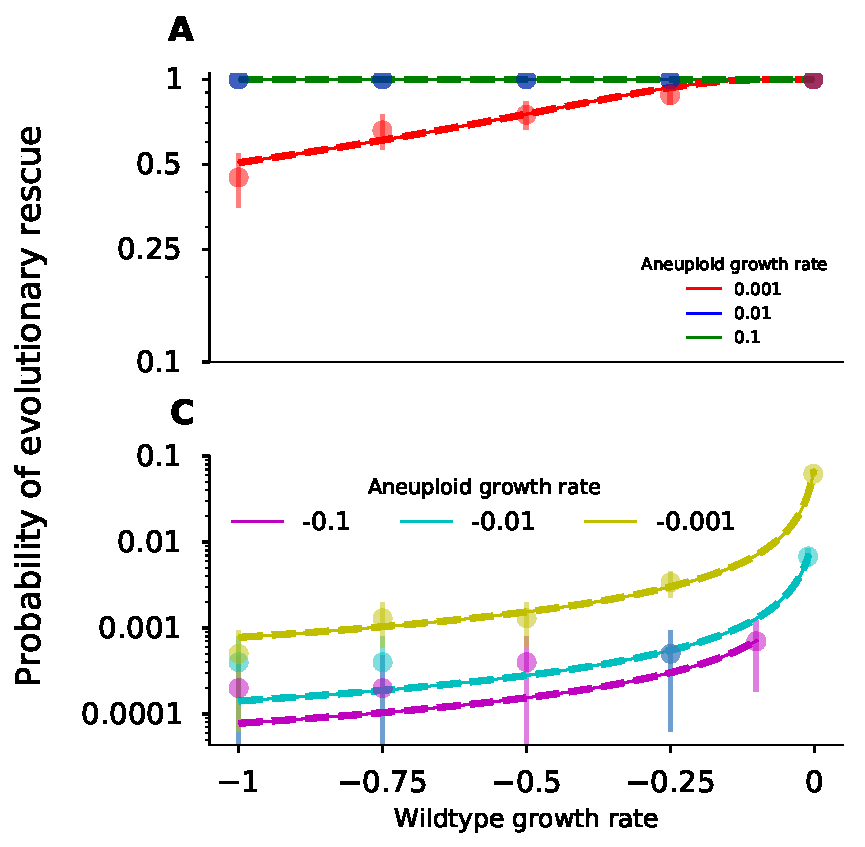
\includegraphics[width=\textwidth]{Figures/CombinedSubplot.pdf}      
%      \label{SurvPlot}
%\end{subfigure}
%\begin{subfigure}{0.5\textwidth}
%      \centering
%      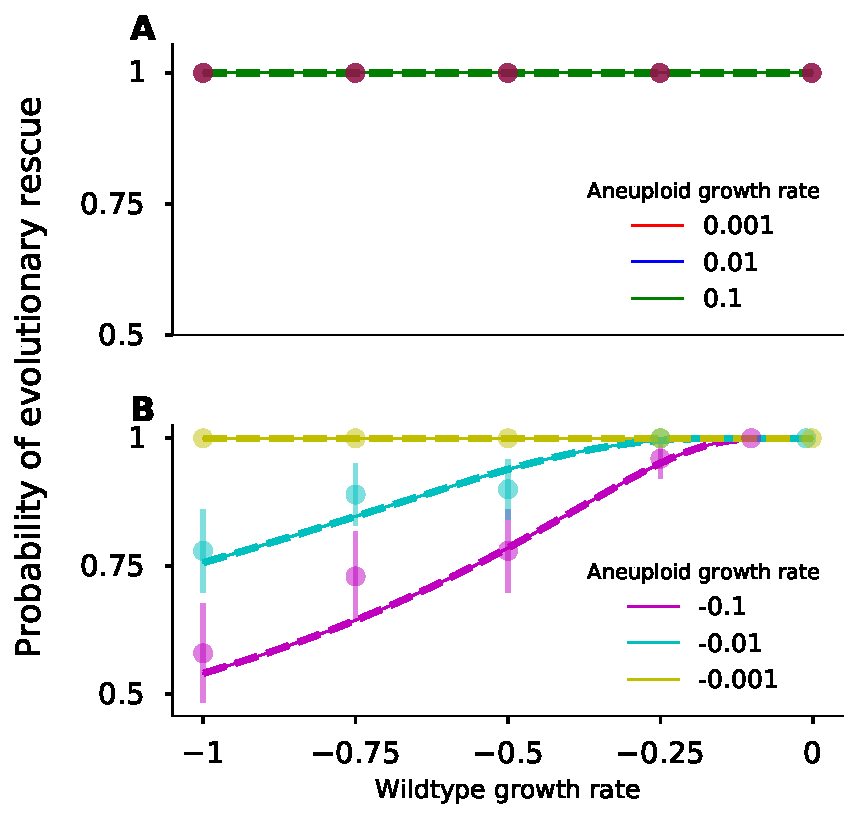
\includegraphics[width=\textwidth]{Figures/CombinedSubplotLargePop.pdf}      
%      \label{SurvPlotLargeN}
%\end{subfigure}
%\caption{Survival probability for large-effect aneuploidy.}
%\label{}
%\end{figure}  
%%%%%%%%%%%
\begin{figure}[p]
% small population size
% A: partial resistance
% B: tolerance
 \vspace*{1\baselineskip}
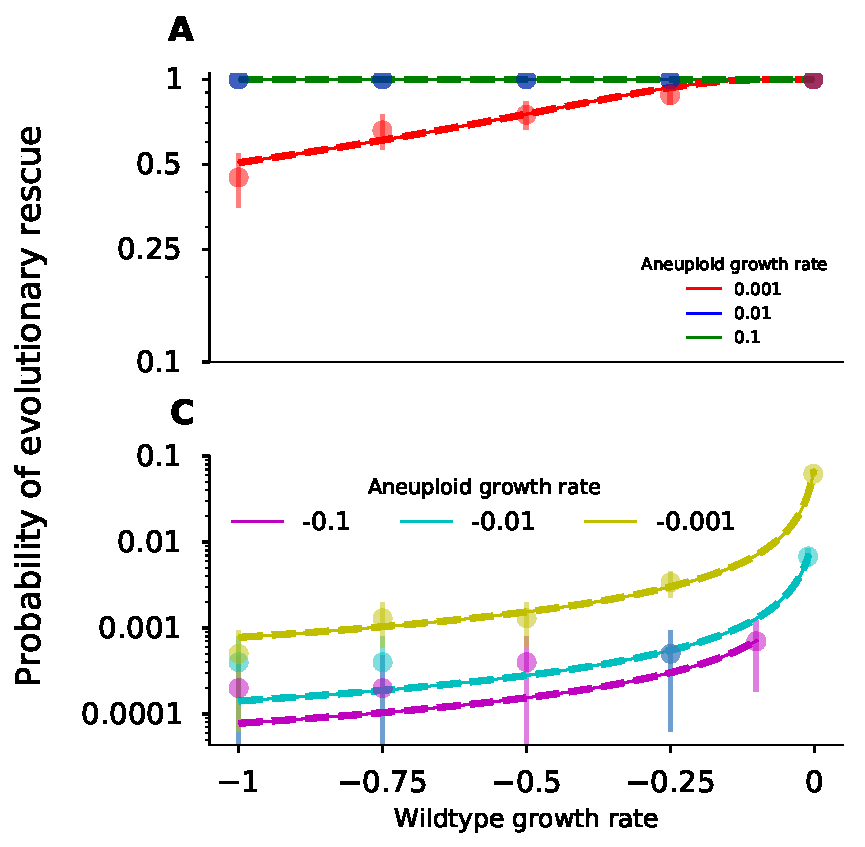
\includegraphics[width=1\textwidth]{Figures/CombinedSubplot.pdf}
\caption{Plot of the probability of evolutionary rescue of a population, consisting initially of $N$ wildtype cells, as a function of the proliferation rate of the wildtype cells for various values of the proliferation rate of the aneuploid cells. The continuous lines represent the exact result \eqref{survprobw} while the dashed lines represent the approximation \eqref{aneuploidyresistentfirstapprox} for the upper plot and \eqref{AneuploidyDeleteriousApprox} for the lower plot. The dots represent numerical simulations where the error bars represent $95\%$ confidence interval of the form $p\pm1.96\sqrt{p\left(1-p\right)/n}$ where $p$ is the mean probability of evolutionary rescue and $n$ is the number of simulations. Here the population initially consists of $N$ wildtype cells and for the simulations we have chosen the following parameters: $N=10^4, \lambda_a=1+10^{-2},\lambda_m=1+10^{-1},\mu_w=1,\mu_a=1,\mu_m=1$. }
\label{SurvPlot}
\end{figure}
%%%%%%%%%%%
\begin{figure}[p]
% large population size
% A: partial resistance
% B: tolerance
 \vspace*{1\baselineskip}
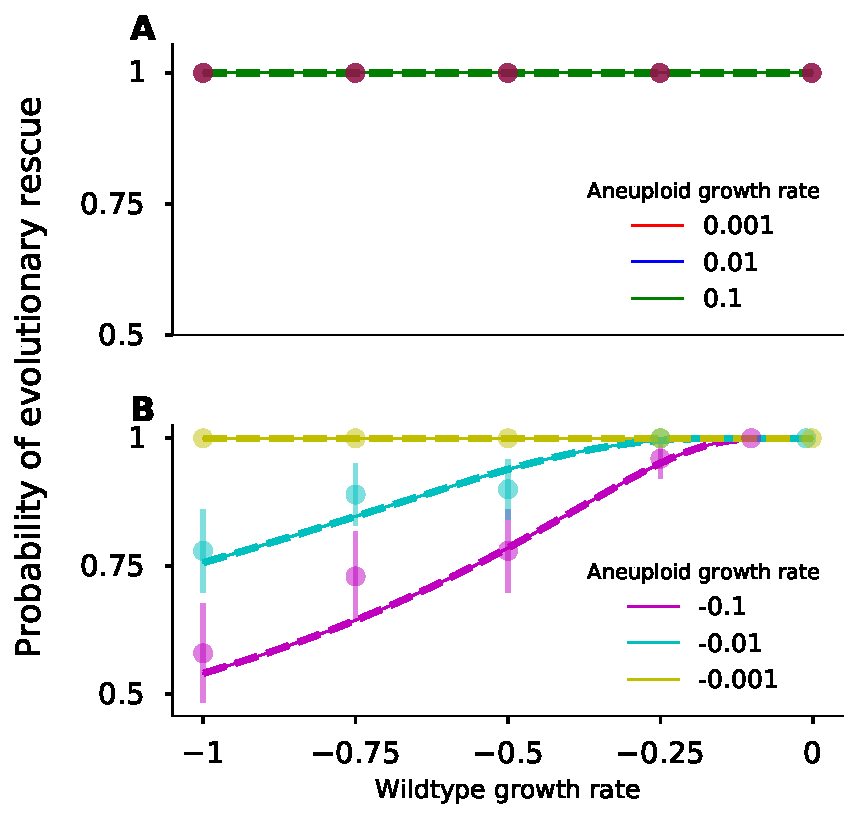
\includegraphics[width=1\textwidth]{Figures/CombinedSubplotLargePop.pdf}
\caption{Plot of the probability of evolutionary rescue of a population, consisting initially of $N$ wildtype cells, as a function of the proliferation rate of the wildtype cells for various values of the proliferation rate of the aneuploid cells. The continuous lines represent the exact result \eqref{survprobw} while the dashed lines represent the approximation \eqref{aneuploidyresistentfirstapprox} for the upper plot and \eqref{AneuploidyDeleteriousApprox} for the lower plot. The dots represent numerical simulations where the error bars represent $95\%$ confidence interval of the form $p\pm1.96\sqrt{p\left(1-p\right)/n}$ where $p$ is the mean probability of evolutionary rescue and $n$ is the number of simulations.  Here the population initially consists of $N$ wildtype cells and for the simulations we have chosen the following parameters: $N=10^8, \lambda_w=0.14, \lambda_a=0.14,\lambda_m=0.14,\mu_m=0.13, u=10^{-2}, v=10^{-7}$. }
\label{SurvPlotLargeN}
\end{figure}
%%%%%%%%%%%
\begin{figure}[p]
% partial resistance, compare 1st and 2nd order approximation and exact
 \vspace*{1\baselineskip}
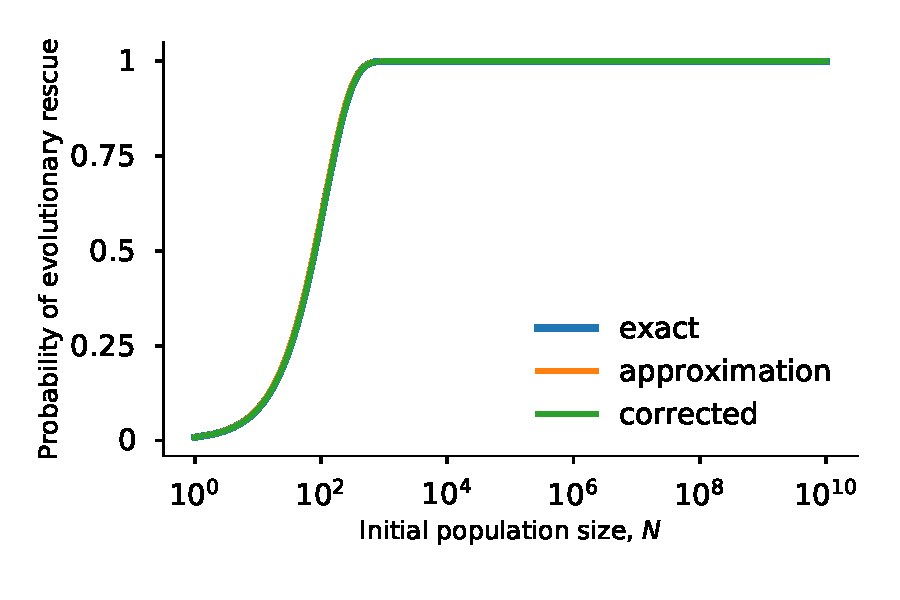
\includegraphics[width=1\textwidth]{Figures/SurvPlotNData.pdf}
\caption{Plot of the probability of survival of a population as a function of the initial population size of wildtype cells. The blue line represents the exact solution \eqref{survprobw}, the orange line line represents the approximation \eqref{aneuploidyresistentfirstapprox}, the green line represents the first order correction \eqref{survprobwapproxcorrected} and the red dots represents stochastic simulations. For the simulations we have chosen the following parameters: $\lambda_w=0.14, \lambda_a=0.14,\lambda_m=0.14,\mu_w=0.17,\mu_a=0.135,\mu_m=0.13$. The error bars represent $95\%$ confidence interval of the form $p\pm1.96\sqrt{p\left(1-p\right)/n}$ where $p$ is the mean probability of evolutionary rescue and $n=100$ is the number of simulations.}
\label{SurvPlotNData}
\end{figure}
%%%%%%%%%%%
\begin{figure}[p]
% small population size
% switch from tolerance to non-growing
 \vspace*{1\baselineskip}
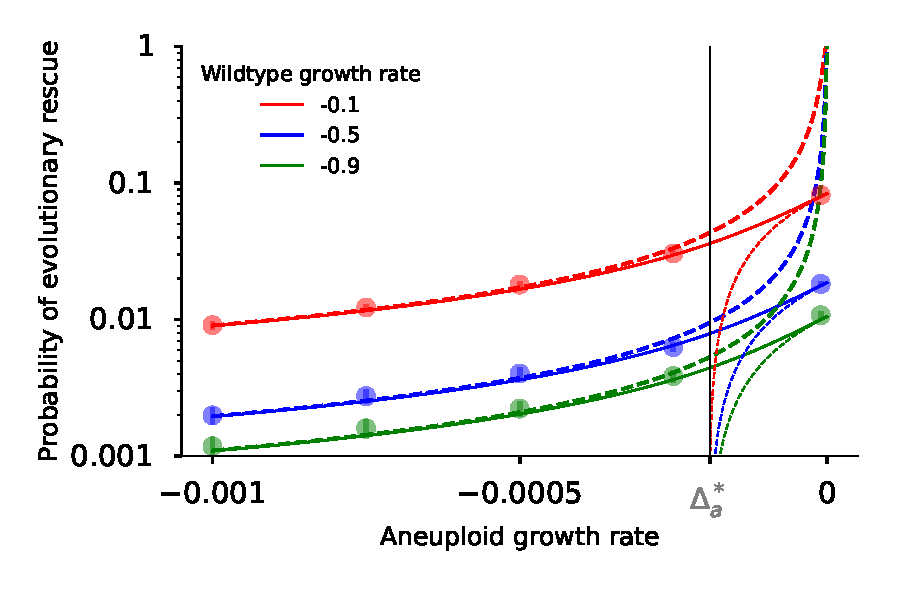
\includegraphics[width=1\textwidth]{Figures/P_est_divergence.pdf}
\caption{Plot of the probability of evolutionary rescue, of an initial population, consisting of $N$ wildtype cells, as a function of proliferation rate of the wildtype cells $\Delta_w=\lambda_w-\mu_w$ for various values of the proliferation rate of the aneuploid cells $\Delta_a=\lambda_a-\mu_a$. The continuous lines represent the exact result \eqref{survprobw} while the dashed lines represent the approximations \eqref{AneuploidyDeleteriousApprox} and \eqref{pestthirdcase}. The dots represent numerical simulations where the error bars represent $95\%$ confidence interval of the form $p\pm1.96\sqrt{p\left(1-p\right)/n}$ where $p$ is the mean probability of evolutionary rescue and $n$ is the number of simulations. The value highlighted in grey is the threshold $\Delta_a^*$ from \eqref{thresholdvalueaneuploid} which marks the transition between the regime dictated by \eqref{AneuploidyDeleteriousApprox} to the one dictated by \eqref{pestthirdcase}.  Here the population initially consists of $N$ wildtype cells and for the simulations we have chosen the following parameters: $N=10^4,\lambda_m=1+10^{-1},\mu_w=1,\mu_a=1,\mu_m=1$. }
\label{P_est}
\end{figure}
%%%%%%%%%%%
\begin{figure}[p]
% large population size
% switch from tolerance to non-growing
 \vspace*{1\baselineskip}
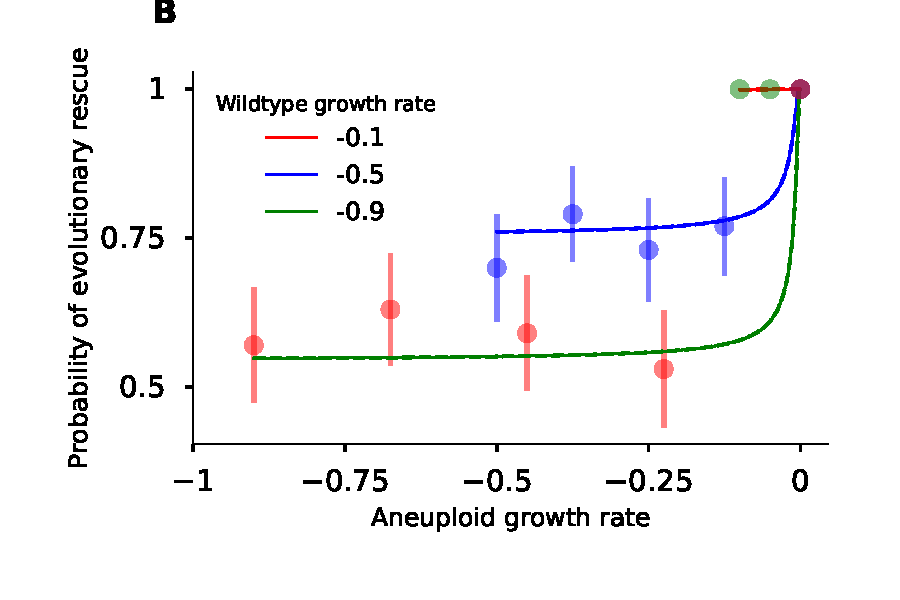
\includegraphics[width=1\textwidth]{Figures/P_est_divergenceLargePopulation.pdf}
\caption{Plot of the probability of evolutionary rescue, of an initial population, consisting of $N$ wildtype cells, as a function of proliferation rate of the wildtype cells $\Delta_w=\lambda_w-\mu_w$ for various values of the proliferation rate of the aneuploid cells $\Delta_a=\lambda_a-\mu_a$. The continuous lines represent the exact result \eqref{survprobw} while the dashed lines represent the approximations \eqref{AneuploidyDeleteriousApprox}. The dots represent numerical simulations where the error bars represent $95\%$ confidence interval of the form $p\pm1.96\sqrt{p\left(1-p\right)/n}$ where $p$ is the mean probability of evolutionary rescue and $n$ is the number of simulations.  Here the population initially consists of $N$ wildtype cells and for the simulations we have chosen the following parameters: $N=10^8,\lambda_m=1+10^{-1},\mu_w=1,\mu_a=1,\mu_m=1$. }
\label{P_est_large_N}
\end{figure}
%%%%%%%%%%%
\begin{figure}[p]
% non-growing slightly declining, compare 1st order approximation to exact and simulation
 \vspace*{1\baselineskip}
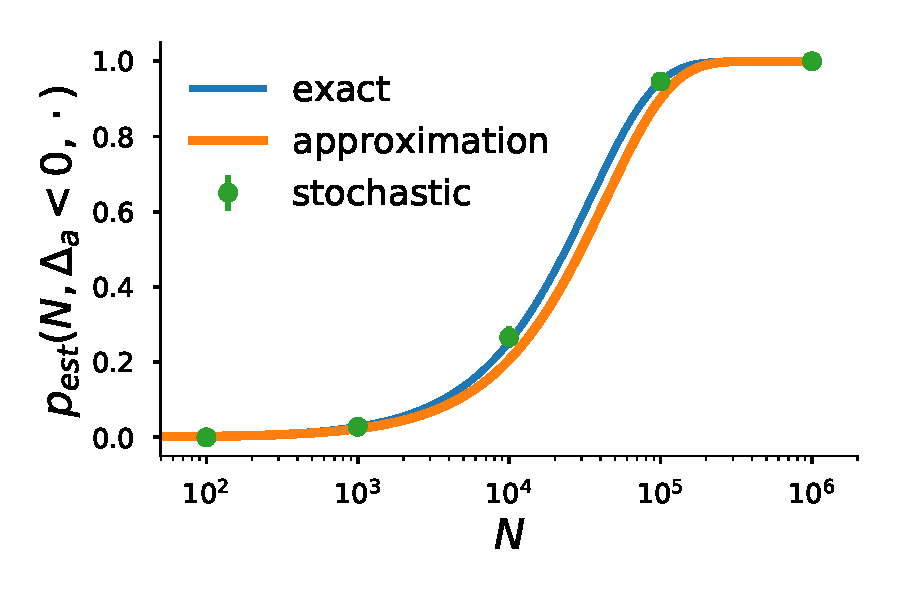
\includegraphics[width=1\textwidth]{Figures/DeleteriousTauLeapPlot.pdf}
\caption{Plot of the probability of evolutionary rescue of a population, consisting of $N$ wildtype cells, as a function of the initial population size of wildtype cells. The blue line represent the exact result \eqref{survprobw} while the orange lines represent the approximation \eqref{pestthirdcase}. The green dots represent numerical simulations where the error bars represent $95\%$ confidence interval of the form $p\pm1.96\sqrt{p\left(1-p\right)/n}$ where $p$ is the mean probability of evolutionary rescue and $n$ is the number of simulations. The error bars are present but are not visible given the fact that we have used $n=10^5$ simulations for each combination of parameters. Here the population initially consists of $N$ wildtype cells and for the simulations we have chosen the following parameters: $\lambda_m=1+10^{-1},\mu_w=1,\mu_a=1,\mu_m=1$.}
\label{DeleteriousPlot}
\end{figure}
%%%%%%%%%%%
\begin{figure}[p]
% density-dependent simulations, barely growing (or maybe partial resistance), with exact formula
 \vspace*{1\baselineskip}
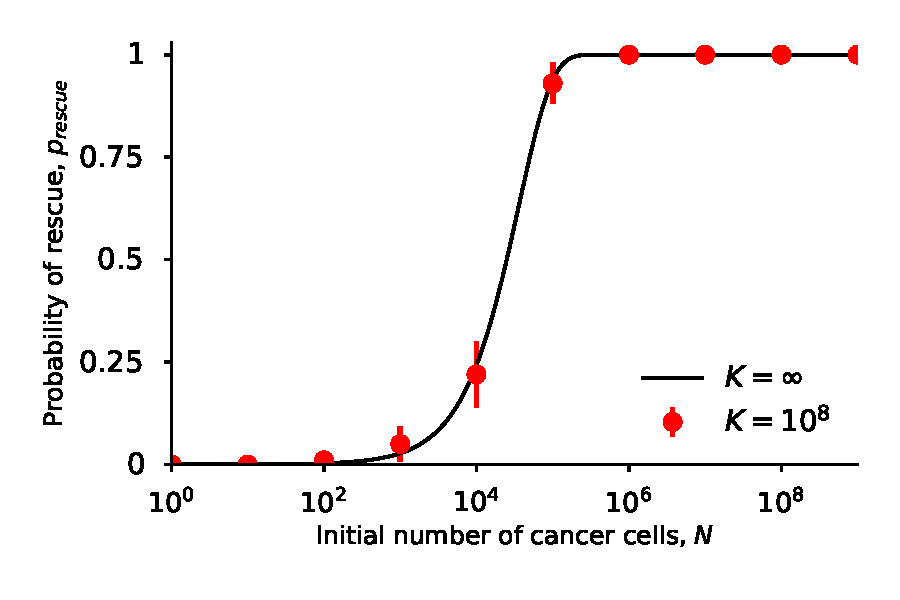
\includegraphics[width=1\textwidth]{Figures/SurvPlotNDataLogisticK.pdf}
\caption{Plot of the probability of evolutionary rescue of a population, consisting of $N$ wildtype cells, as a function of the initial population size of wildtype cells where maximum population size is constrained by the carrying capacity $K$.  The blue line represent the exact result \eqref{survprobw} while the orange dots represent numerical simulations where the error bars represent $95\%$ confidence interval of the form $p\pm1.96\sqrt{p\left(1-p\right)/n}$ where $p$ is the mean probability of evolutionary rescue and $n$ is the number of simulations. Here the population initially consists of $N$ wildtype cells and for the simulations we have chosen the following parameters: $\lambda_w=1-10^{-1},\lambda_a=1+10^{-4},\lambda_m=1+10^{-1},\mu_w=1,\mu_m=1,u=10^{-2},v=10^{-7}, C_1=C_2=1, K=10^9$.}
\label{SurvPlotNDataLogisticKComplete}
\end{figure}
%%%%%%%%%%%
\begin{figure}[p]
% A partial resistance
% B tolerance
% function of wildtype growth rate
 \vspace*{1\baselineskip}
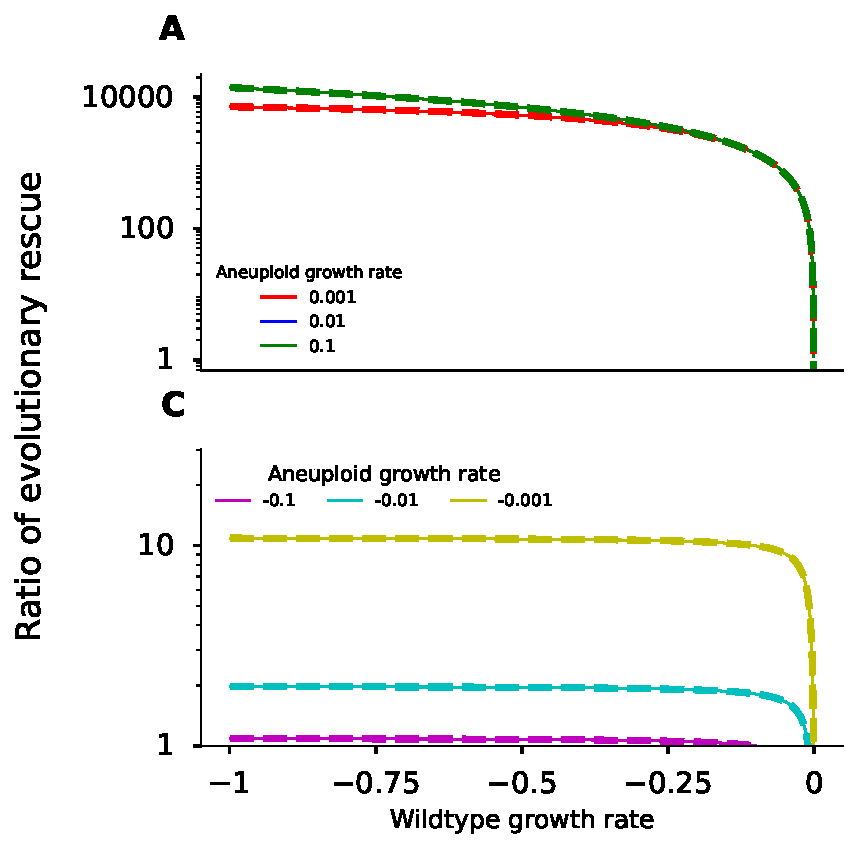
\includegraphics[width=1\textwidth]{Figures/RatioEvolRescue.pdf}
\caption{Plot of the ratio of the probability of evolutionary rescue when aneuploidy can play a role in rescue ($u>0$) to the probability where acquisition of aneuploidy is not possible ($u=0$) as a function of the proliferation rate of the wildtype cells. The continuous lines represent the exact result \eqref{ratiorescueexact} while the dashed lines represent the approximation \eqref{ratiorescue}.  The upper plot show the case when aneuploidy is resistant while the lower plot shows the case when it is susceptible. Here the population initially consists of $N$ wildtype cells and for the simulations we have chosen the following parameters: $\lambda_w=1-10^{-1},\lambda_m=1+10^{-1},\mu_w=1,\mu_a=1,\mu_m=1$. }
\label{RatioEvolRescue}
\end{figure}
%%%%%%%%%%%
\begin{figure}[p]
% A partial resistance
% B tolerance
% function of population size
 \vspace*{1\baselineskip}
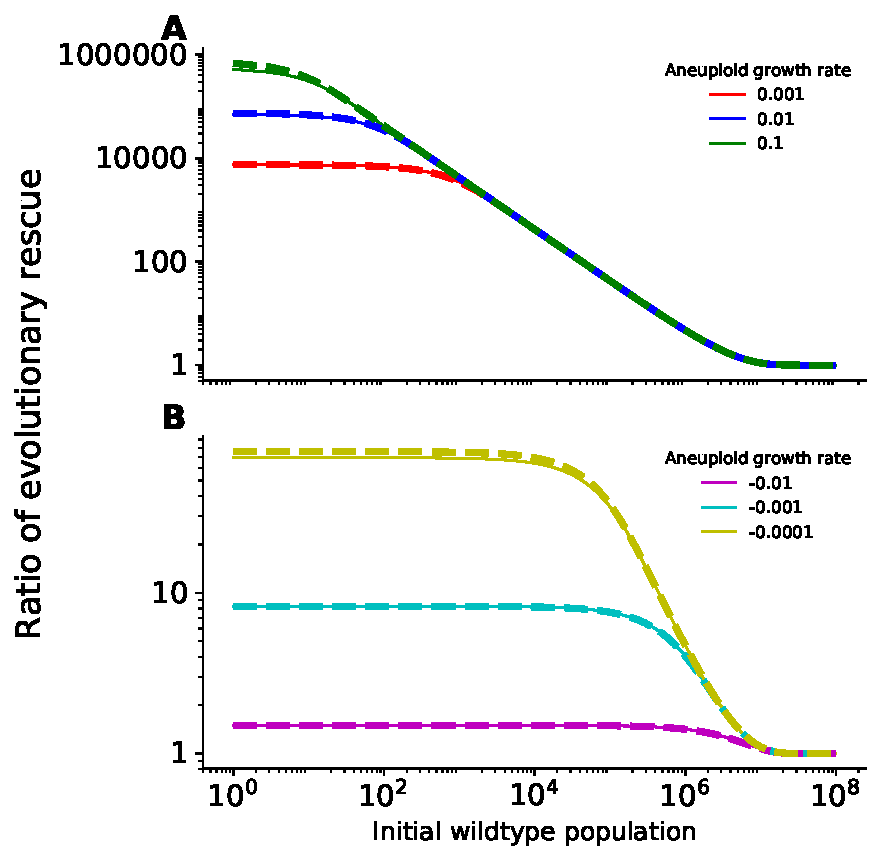
\includegraphics[width=1\textwidth]{Figures/RatioEvolRescuePopulationSize.pdf}
\caption{Plot of the ratio of the probability of evolutionary rescue when aneuploidy can play a role in rescue ($u>0$) to the probability where acquisition of aneuploidy is not possible ($u=0$) as a function of the initial population size of wildtype cells. The continuous lines represent the exact result \eqref{ratiorescueexact} while the dashed lines represent the approximation \eqref{ratiorescue}. The upper plot show the case when aneuploidy is resistant while the lower plot shows the case when it is susceptible.  Here the population initially consists of $N$ wildtype cells and for the simulations we have chosen the following parameters: $\lambda_w=0.14, \lambda_a=0.14,\lambda_m=0.14,\mu_w=0.17,\mu_m=0.13, u=10^{-2}, v=10^{-7}$. }
\label{RatioEvolRescuePopulationSize}
\end{figure}
%%%%%%%%%%%
\begin{figure}[p]
% partial resistance - aneuploidy rescues the pop
 \vspace*{1\baselineskip}
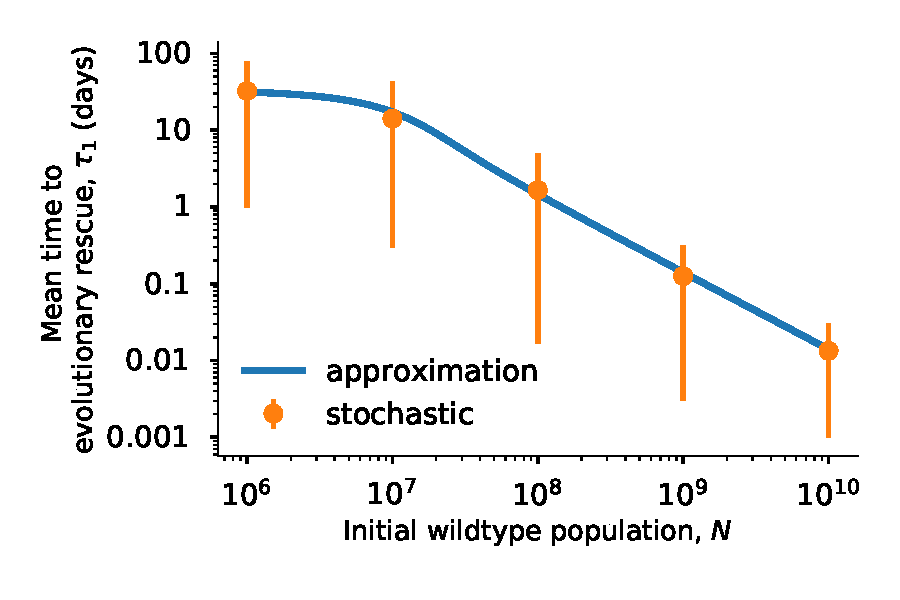
\includegraphics[width=1\textwidth]{Figures/MeanTimeGrowthMutantDirectPlot.pdf}
\caption{Plot of the mean time until the appearance of a resistance mutation which rescues the population in the case when evolutionary rescue is possible only through mutation but not aneuploidy and mutation.  The blue line represents the approximation \eqref{meantime1} and the dashed red line represents the first order approximation \eqref{limitapprox}. The orange dots represent the numerical simulations while the error bars represent the interval centered at the mean which containing $95\%$ of the simulated values. Here the population initially consists of $N$ wildtype cells and for the simulations we have chosen the following parameters: $\lambda_w=1-10^{-1},\lambda_m=1+10^{-1},\mu_w=1,\mu_m=1,u=10^{-2},v=10^{-7}$.}
\label{MeanTimeGrowthAneuploidyPlot}
\end{figure}
%%%%%%%%%%%
\begin{figure}[p]
% slightly decreasing (need to check)
 \vspace*{1\baselineskip}
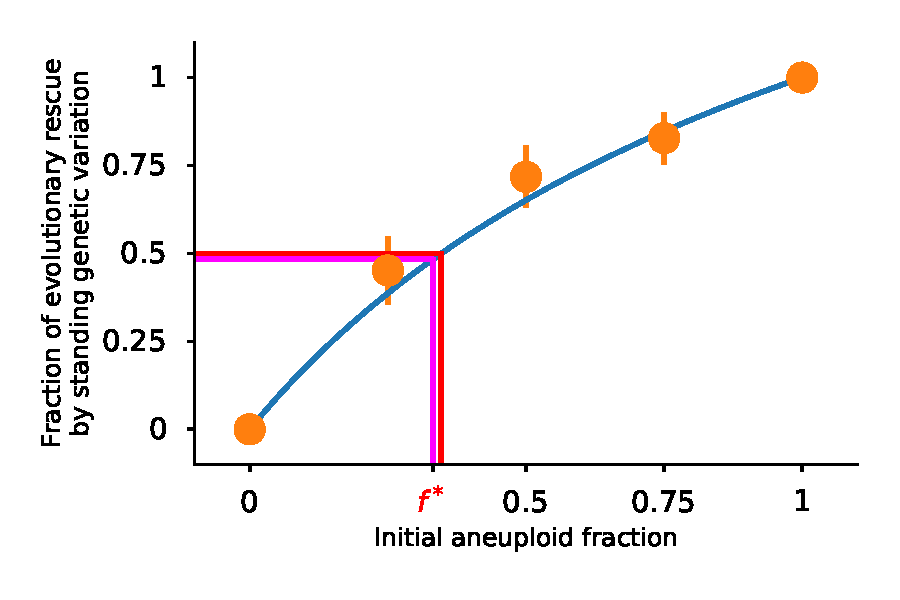
\includegraphics[width=1\textwidth]{Figures/FractionPlot.pdf}
\caption{Plot of the fraction of the cases the population is rescue by standing genetic variation as a function of the fraction of initial cells which are aneuploid. The red vertical line highlights the the value of $f$ for which half the times the population is rescues by aneuploid cells while the pink line is our approximation \eqref{halfeqstandvar}. For this plot we have chosen the following parameters: $N=10^3, \lambda_w=1-10^{-2}, \lambda_a=1-10^{-4},\lambda_m=1+10^{-1},\mu_w=1,\mu_a=1,\mu_m=1$. The error bars represent $95\%$ confidence interval of the form $p\pm1.96\sqrt{p\left(1-p\right)/n}$ where $p$ is the mean probability of evolutionary rescue and $n$ is the number of simulations. The value of $0.332$ highlighted in red is the value of the initial fraction of the population which in aneuploid for which half of the cases of evolutionary rescue are due to the initial aneuploid cell population.}
\label{FractionPlot}
\end{figure}
%%%%%%%%%%%
\begin{figure}[p]
% tolerance
 \vspace*{1\baselineskip}
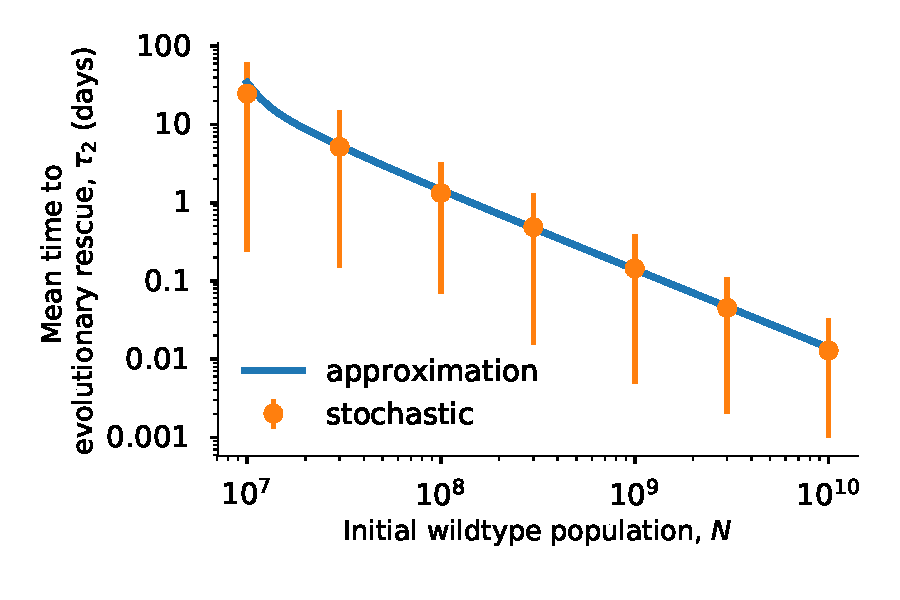
\includegraphics[width=1\textwidth]{Figures/MeanTimeDeleteriousPlot.pdf}
\caption{Plot of the mean time until the appearance of a resistance mutation which rescues the population in the case when evolutionary rescue is possible 
 through mutation and aneuploidy.  Here the population initially consists of $N$ wildtype cells and for the simulations we have chosen the following parameters: $\lambda_w=1-10^{-1},\lambda_a=1-10^{-2},\lambda_m=1+10^{-1},\mu_w=1,\mu_a=1,\mu_m=1,u=10^{-2},v=10^{-7}$.  The blue line represents the approximation \eqref{meantimet2}, the dashed red line represents the second order approximation \eqref{limitapprox2} and the green line is first order approximation \eqref{limitapprox3}. The orange dots represent the numerical simulations while the error bars represent the interval centered at the mean which containing $95\%$ of the simulated values.}
\label{MeanTimeDeleteriousAneuploidyPlot}
\end{figure}
%%%%%%%%%%%
\begin{figure}[p]
% tolerance... maybe third is slightly decreasing
 \vspace*{1\baselineskip}
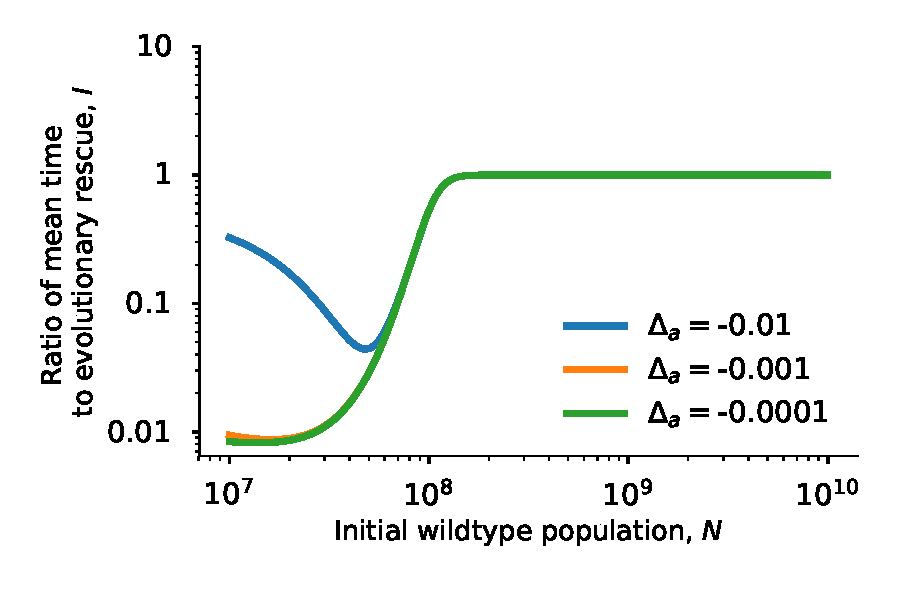
\includegraphics[width=1\textwidth]{Figures/MeanTimeRatioInitialPopulationSize.pdf}
\caption{Plot of the ratio of the mean time to evolutionary rescue when aneuploidy can play a role in rescue ($u>0$) to the mean time where acquisition of aneuploidy is not possible ($u=0$) as a function of the initial population size of wildtype cells. The continuous lines represent the approximation \eqref{eqMeanTimeRatioInitialPopulationSize}.  Here the population initially consists of $N$ wildtype cells and for the simulations we have chosen the following parameters: $\lambda_w=1-10^{-1},\lambda_m=1+10^{-1},\mu_w=1,\mu_a=1,\mu_m=1$.}
\label{MeanTimeRatioInitialPopulationSize}
\end{figure}
%%%%%%%%%%%
\begin{figure}[p]
% diffusion approx instead of branching process
% tolerance
 \vspace*{1\baselineskip}
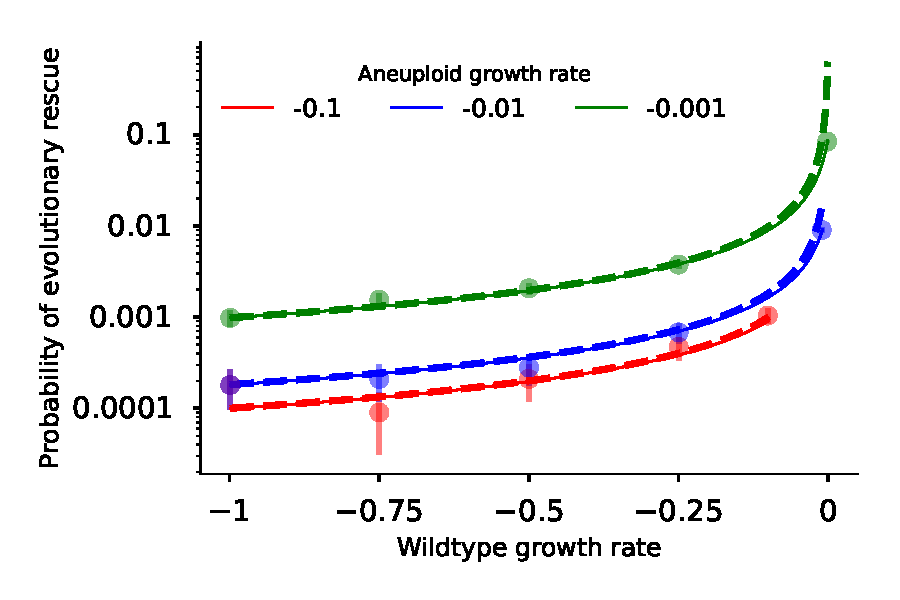
\includegraphics[width=1\textwidth]{Figures/P_est_diffusion.pdf}
\caption{Plot of the survival probability of an initial population consisting of $w_0=10^{4}$ wildtype cells as a function of $\Delta_a=\lambda_a-\mu_a$ for various values of $\Delta_w=\lambda_a-\mu_a$. The continuous lines represent the exact result \eqref{survprobw} while the dashed lines represent the Feller diffusion approximation \eqref{FellerApprox}. The error bars represent $95\%$ confidence interval of the form $p\pm1.96\sqrt{p\left(1-p\right)/w_0}$ where $p$ is the mean probability of evolutionary rescue.}
\label{P_est_diffusion}
\end{figure}
%%%%%%%%%%%%%%%%%%%%%%%%%%%%%%%%%%%%%%%%%%
%\appendix
\begin{appendices}
\renewcommand{\theequation}{\thesection\arabic{equation}}
\counterwithin*{equation}{section}

%%%%%%%%%%%%%%%%%%%%%%%%%%%%%%%%%%%%%%%%%%
%\section*{Gillespie algorithm}
%\begin{subequations}
%\begin{flalign}
%(+1,0,0)&:\quad \lambda_ww_t,\\
%(-1,0,0)&:\quad \mu_ww_t,\\
%(-1,+1,0)&:\quad uw_t,\\
%(-1,0,+1)&:\quad vw_t,\\
%(0,+1,0)&:\quad \lambda_aa_t,\\
%(0,-1,0)&:\quad \mu_aa_t,\\
%(0,-1,+1)&:\quad va_t,\\
%(0,0,+1)&:\quad \lambda_am_t,\\
%(0,0,-1)&:\quad \mu_am_t.
%\end{flalign}
%\end{subequations}

%%%%%%%%%%%%%%%%%%%%%%%%%%%%%%%%%%%%%%%%%%
%%%%%%%%%%%%%%%%%%%%%%%%%%%%%%%%%%%%%%%%%%
%\section*{Mean time}
%%%%%%%%%%%%%%%%%%%%%%%%%%%%%%%%%%%%%%%%%%%
%We define the following events
%\begin{align*}
%\text{EvR}&=\text{``evolutionary rescue occurs''},\\
%\text{EvRA}&=\text{``evolutionary rescue occurs through aneuploidy''},\\
%\text{EvRM}&=\text{``evolutionary rescue occurs through mutation''}.
%\end{align*}
%As a result, the mean time to appearence of the first mutant cell which rescues the population given evolutionary rescue can be expanded as:
%\begin{align*}
%\mathbb{E}\left[\tau|\text{EvR}\right]&=\mathbb{E}\left[\tau|\text{EvR},\text{EvRA}\cap\text{EvRM}^{C}\right]p\left(\text{EvRA}\cap\text{EvRM}^{C}|\text{EvR}\right)\\
%&+\mathbb{E}\left[\tau|\text{EvR},\text{EvRM}\cap\text{EvRA}^{C}\right]p\left(\text{EvRM}\cap\text{EvRA}^{C}|\text{EvR}\right)\\
%&+\mathbb{E}\left[\tau|\text{EvR},\text{EvRM}\cap\text{EvRA}\right]p\left(\text{EvRM}\cap\text{EvRA}|\text{EvR}\right).
%\end{align*}
%The joint probabilities in the previous lines can be written as:
%\begin{align*}
%p\left(\text{EvRA}\cap\text{EvRM}^{C}|\text{EvR}\right)&=\frac{p\left(\text{EvRA}\cap\text{EvRM}^{C}\right)}{p\left(\text{EvR}\right)}
%\approx\frac{p\left(\text{EvRA}\right)\left[1-p\left(\text{EvRM}\right)\right]}{p\left(\text{EvR}\right)},\\
%p\left(\text{EvRM}\cap\text{EvRA}^{C}|\text{EvR}\right)&=\frac{p\left(\text{EvRM}\cap\text{EvRA}^{C}\right)}{p\left(\text{EvR}\right)}
%\approx\frac{p\left(\text{EvRM}\right)\left[1-p\left(\text{EvRA}\right)\right]}{p\left(\text{EvR}\right)},\\
%p\left(\text{EvRM}\cap\text{EvRA}|\text{EvR}\right)&=\frac{p\left(\text{EvRM}\cap\text{EvRA}\right)}{p\left(\text{EvR}\right)}\approx\frac{p\left(\text{EvRM}\right)p\left(\text{EvRA}\right)}{p\left(\text{EvR}\right)}\ll1.
%\end{align*}
%As a result, we have:
%\begin{align*}
%\mathbb{E}\left[\tau|\text{EvR}\right]&\approx\mathbb{E}\left[\tau|\text{EvR},\text{EvRA}\cap\text{EvRM}^{C}\right]p\left(\text{EvRA}\cap\text{EvRM}^{C}|\text{EvR}\right)\\
%&+\mathbb{E}\left[\tau|\text{EvR},\text{EvRM}\cap\text{EvRA}^{C}\right]p\left(\text{EvRM}\cap\text{EvRA}^{C}|\text{EvR}\right).
%\end{align*}
%%%
%%%%%%%%%%%%%%%%%%%%%%%%%%%%%%%%%%%%%%%%%%
\section*{Diffusion approximation}\label{AppendixDiffApprox}
%%%%%%%%%%%%%%%%%%%%%%%%%%%%%%%%%%%%%%%%%%
An alternative method to obtain the probability of evolutionary rescue is to utilize a Feller diffusion approximation which is governed by two parameters: the growth rate $r$ and the reproductive variance $\sigma$. The two parameters are obtained from the underlying demographic process as the infinitesimal relative change in mean and variance of $n_t$ over and an infinitesimally small time interval $\Delta t$:
\begin{align*}
r&=\lim_{\Delta t\rightarrow0}\frac{\mathbb{E}\left(\Delta n_t|n_t\right)}{\Delta_t n_t},\\
\sigma&=\lim_{\Delta t\rightarrow0}\frac{\mathbb{V}ar\left(\Delta n_t|n_t\right)}{\Delta_t n_t}.
\end{align*}
The rate at which mutants are generated directly from the wildtype is: 
\begin{align}
\theta_1=v\bar{\pi}_f\frac{N}{|r_w|},
\end{align}
where
\begin{align}
\bar{\pi}_f=\int_{0}^\infty\int_{0}^\infty \left(1-\e^{-\frac{2r}{\sigma}}\right) f_r\left(r,\sigma\right)\d r\d\sigma.
\end{align}
Letting $f_r\left(r,\sigma\right)=\delta\left(r-r_m\right)\delta\left(\sigma-\sigma_m\right)$ then:
\begin{align}
\bar{\pi}_f=1-\e^{-\frac{2r_m}{\sigma_m}},
\end{align}
and, as a result, we have:
\begin{align}
\theta_1=v\left(1-\e^{-\frac{2r_m}{\sigma_m}}\right)\frac{N}{|\Delta_w|}.
\end{align}
The rate at which mutants are generated indirectly from the wildtype through aneuploidy is: 
\begin{align*}
\theta_2&=\frac{uN}{|r_w|}\int_{0}^\infty\int_{0}^\infty \left(1-\pi_f\left(r,q\right)\right) f_r\left(r,\sigma\right) p_1^*\left(r,\sigma\right)\d r\d\sigma\\
&=\frac{uN}{|\Delta_w|}p_1^*\left(r_a,\sigma_a\right)\\
&=\frac{uN}{|\Delta_w|}\left[1-\exp\left(-\frac{|r_a|}{\sigma_a^2}\left(\sqrt{1+\frac{2\sigma_a^2}{r_a^2}u^*}-1\right)\right)\right]\\
&=\frac{uN}{|\Delta_w|}\left[1-\exp\left(-\frac{|\Delta_a|}{(\lambda_a+\mu_a)^2}\left(\sqrt{1+\frac{2(\lambda_a+\mu_a)^2}{\Delta_a^2}u^*}-1\right)\right)\right],
\end{align*}
where
\begin{equation}
u^*=v\left(1-\e^{-\frac{2r_m}{\sigma_m}}\right).
\end{equation}
The number of rescue mutations has a Poisson distribution with rate $\theta_1+\theta_2$. As a result, the probability of evolutionary rescue is given by:
\begin{equation}\label{FellerApprox}
p_{rescue}=1-\e^{-\left(\theta_1+\theta_2\right)},
\end{equation}
which we plot in Figure \ref{P_est_diffusion} as a function of $\Delta_w$.
\end{appendices}

%%%%%%%%%%%%%%%%%%%%%%%%%%%%%%%%%%%%%%%%%%
\end{document}